\documentclass[dvipdfmx]{jsarticle}
\setcounter{section}{2}
\setcounter{subsection}{4}
\usepackage{xr}
\externaldocument{2.2.1}
\externaldocument{2.2.2}
\externaldocument{2.2.4}
\usepackage{amsmath,amsfonts,amssymb,array,comment,mathtools,url,docmute}
\usepackage{longtable,booktabs,dcolumn,tabularx,mathtools,multirow,colortbl,xcolor}
\usepackage[dvipdfmx]{graphics}
\usepackage{bmpsize}
\usepackage{amsthm}
\usepackage{enumitem}
\setlistdepth{20}
\renewlist{itemize}{itemize}{20}
\setlist[itemize]{label=•}
\renewlist{enumerate}{enumerate}{20}
\setlist[enumerate]{label=\arabic*.}
\setcounter{MaxMatrixCols}{20}
\setcounter{tocdepth}{3}
\newcommand{\rotin}{\text{\rotatebox[origin=c]{90}{$\in $}}}
\newcommand{\amap}[6]{\text{\raisebox{-0.7cm}{\begin{tikzpicture} 
  \node (a) at (0, 1) {$\textstyle{#2}$};
  \node (b) at (#6, 1) {$\textstyle{#3}$};
  \node (c) at (0, 0) {$\textstyle{#4}$};
  \node (d) at (#6, 0) {$\textstyle{#5}$};
  \node (x) at (0, 0.5) {$\rotin $};
  \node (x) at (#6, 0.5) {$\rotin $};
  \draw[->] (a) to node[xshift=0pt, yshift=7pt] {$\textstyle{\scriptstyle{#1}}$} (b);
  \draw[|->] (c) to node[xshift=0pt, yshift=7pt] {$\textstyle{\scriptstyle{#1}}$} (d);
\end{tikzpicture}}}}
\newcommand{\twomaps}[9]{\text{\raisebox{-0.7cm}{\begin{tikzpicture} 
  \node (a) at (0, 1) {$\textstyle{#3}$};
  \node (b) at (#9, 1) {$\textstyle{#4}$};
  \node (c) at (#9+#9, 1) {$\textstyle{#5}$};
  \node (d) at (0, 0) {$\textstyle{#6}$};
  \node (e) at (#9, 0) {$\textstyle{#7}$};
  \node (f) at (#9+#9, 0) {$\textstyle{#8}$};
  \node (x) at (0, 0.5) {$\rotin $};
  \node (x) at (#9, 0.5) {$\rotin $};
  \node (x) at (#9+#9, 0.5) {$\rotin $};
  \draw[->] (a) to node[xshift=0pt, yshift=7pt] {$\textstyle{\scriptstyle{#1}}$} (b);
  \draw[|->] (d) to node[xshift=0pt, yshift=7pt] {$\textstyle{\scriptstyle{#2}}$} (e);
  \draw[->] (b) to node[xshift=0pt, yshift=7pt] {$\textstyle{\scriptstyle{#1}}$} (c);
  \draw[|->] (e) to node[xshift=0pt, yshift=7pt] {$\textstyle{\scriptstyle{#2}}$} (f);
\end{tikzpicture}}}}
\renewcommand{\thesection}{第\arabic{section}部}
\renewcommand{\thesubsection}{\arabic{section}.\arabic{subsection}}
\renewcommand{\thesubsubsection}{\arabic{section}.\arabic{subsection}.\arabic{subsubsection}}
\everymath{\displaystyle}
\allowdisplaybreaks[4]
\usepackage{vtable}
\theoremstyle{definition}
\newtheorem{thm}{定理}[subsection]
\newtheorem*{thm*}{定理}
\newtheorem{dfn}{定義}[subsection]
\newtheorem*{dfn*}{定義}
\newtheorem{axs}[dfn]{公理}
\newtheorem*{axs*}{公理}
\renewcommand{\headfont}{\bfseries}
\makeatletter
  \renewcommand{\section}{%
    \@startsection{section}{1}{\z@}%
    {\Cvs}{\Cvs}%
    {\normalfont\huge\headfont\raggedright}}
\makeatother
\makeatletter
  \renewcommand{\subsection}{%
    \@startsection{subsection}{2}{\z@}%
    {0.5\Cvs}{0.5\Cvs}%
    {\normalfont\LARGE\headfont\raggedright}}
\makeatother
\makeatletter
  \renewcommand{\subsubsection}{%
    \@startsection{subsubsection}{3}{\z@}%
    {0.4\Cvs}{0.4\Cvs}%
    {\normalfont\Large\headfont\raggedright}}
\makeatother
\makeatletter
\renewenvironment{proof}[1][\proofname]{\par
  \pushQED{\qed}%
  \normalfont \topsep6\p@\@plus6\p@\relax
  \trivlist
  \item\relax
  {
  #1\@addpunct{.}}\hspace\labelsep\ignorespaces
}{%
  \popQED\endtrivlist\@endpefalse
}
\makeatother
\renewcommand{\proofname}{\textbf{証明}}
\usepackage{tikz,graphics}
\usepackage[dvipdfmx]{hyperref}
\usepackage{pxjahyper}
\hypersetup{
 setpagesize=false,
 bookmarks=true,
 bookmarksdepth=tocdepth,
 bookmarksnumbered=true,
 colorlinks=false,
 pdftitle={},
 pdfsubject={},
 pdfauthor={},
 pdfkeywords={}}
\begin{document}
%\hypertarget{ux51aaux96f6ux5909ux63db}{%
\subsection{冪零変換}%\label{ux51aaux96f6ux5909ux63db}}
%\hypertarget{ux51aaux96f6ux5909ux63db-1}{%
\subsubsection{冪零変換}%\label{ux51aaux96f6ux5909ux63db-1}}
\begin{dfn}
代数的閉体$K$上のvector空間$V$、線形写像$f:V \rightarrow V$が与えられたとき、$\exists l \in \mathbb{N}$に対し、$f^{l} = 0$が成り立つようなその線形写像$f$をそのvector空間$V$の冪零変換という。
\end{dfn}
\begin{thm}\label{2.2.5.1}
代数的閉体$K$上の$n$次元vector空間$V$の線形写像$f$が与えられたとき、その線形写像$f$がそのvector空間$V$の冪零変換であるならそのときに限り、その線形写像$f$の固有多項式$\varPhi_{f}$が次式のように与えられる。
\begin{align*}
\varPhi_{f} = X^{n}
\end{align*}
\end{thm}
\begin{proof}
代数的閉体$K$上の$n$次元vector空間$V$の線形写像$f$が与えられたとき、その線形写像$f$がそのvector空間$V$の冪零変換であるなら、$\exists l \in \mathbb{N}$に対し、$f^{l} = 0$が成り立つことになる。ここで、その線形写像$f$の表現行列の1つを$A$とし、線形写像$L_{A}:K^{n} \rightarrow K^{n};\mathbf{v} \mapsto A\mathbf{v}$の任意の固有値$\lambda$に対するその線形写像$L_{A}$の固有vector$\mathbf{w}$が与えられれば、$\forall n \in \mathbb{N}$に対し、Frobeniusの定理より$A^{n}\mathbf{w} = L_{A}^{n}\left( \mathbf{w} \right) = \lambda^{n}\mathbf{w}$が成り立つ。$n = l$のとき、定理\ref{2.1.5.1}より線形同型写像$\varphi:K^{n} \rightarrow V$が存在して$L_{A} = \varphi^{- 1} \circ f \circ \varphi$が成り立つので、数学的帰納法により次のようになり、
\begin{align*}
L_{A}^{l}\left( \mathbf{w} \right) &= \left( \varphi^{- 1} \circ f \circ \varphi \right)^{l}\left( \mathbf{w} \right)\\
&= \left( \varphi^{- 1} \circ f^{l} \circ \varphi \right)\left( \mathbf{w} \right)\\
&= \varphi^{- 1}\left( f^{l}\left( \varphi\left( \mathbf{w} \right) \right) \right)\\
&= \varphi^{- 1}\left( \mathbf{0} \right) = \mathbf{0}
\end{align*}
したがって、その行列$A$は零行列である。これにより、$\lambda^{l}\mathbf{w} = \mathbf{0}$が成り立つ。ここで、そのvector$\mathbf{w}$は固有vectorであるから、$\lambda = 0$が成り立つ。$L_{A} = \varphi^{- 1} \circ f \circ \varphi$が成り立つことに注意すれば、したがって、その線形写像$L_{A}$の固有多項式$\varPhi_{L_{A}}$は$n$次単位行列$I_{n}$を用いて定理\ref{2.2.2.5}、定理\ref{2.2.2.9}より次式のように与えられる。
\begin{align*}
\varPhi_{f} = \varPhi_{L_{A}} = X^{n}
\end{align*}\par
逆に、その線形写像$f$の固有多項式$\varPhi_{f}$が次式のように与えられたらば、
\begin{align*}
\varPhi_{f} = X^{n}
\end{align*}
Hamilton-Cayleyの定理より次のようになる。
\begin{align*}
\varPhi_{f}(f) = f^{n} = 0
\end{align*}
これにより、その線形写像$f$がそのvector空間$V$の冪零変換である。
\end{proof}
\begin{dfn}
代数的閉体$K$上の$n$次元vector空間$V$の冪零変換$f$が与えられたとき、$f^{l} = 0$なる自然数のうちもっとも小さいものをその冪零変換$f$の指数という。
\end{dfn}
%\hypertarget{halmosux306eux5b9aux7406}{%
\subsubsection{Halmosの定理}%\label{halmosux306eux5b9aux7406}}
\begin{thm}[Halmosの定理]\label{2.2.5.2}
体$K$上の$n$次元vector空間$V$の指数$q$の冪零変換$f$が与えられたとき、$f^{q - 1}\left( \mathbf{v}_{*} \right) \neq \mathbf{0}$なるvector$\mathbf{v}_{*}$を用いれば、次のことが成り立つ。
\begin{itemize}
\item
  この族$\left\{ f^{i - 1}\left( \mathbf{v}_{*} \right)\right\}_{i\in \varLambda_q } $は線形独立である。
\item
  部分空間${\mathrm{span}}\left\{ f^{i - 1}\left( \mathbf{v}_{*} \right) \right\}_{i \in \varLambda_{q}}$は$f$-不変である。
\item
  $V = {\mathrm{span}}\left\{ f^{i - 1}\left( \mathbf{v}_{*} \right) \right\}_{i \in \varLambda_{q}} \oplus W$なるそのvector空間$V$の$f$-不変な部分空間$W$が存在する。
\end{itemize}
この定理をHalmosの定理という\footnote{ただし、要出典ですね(?)}。
\end{thm}
\begin{proof}
体$K$上の$n$次元vector空間$V$の指数$q$の冪零変換$f$が与えられたとき、$f^{q - 1}\left( \mathbf{v}_{*} \right) \neq 0$なるvector$\mathbf{v}_{*}$を用いて$\sum_{i \in \varLambda_{q}} {c_{i}f^{i - 1}\left( \mathbf{v}_{*} \right)} = \mathbf{0}$とおかれれば、したがって、次のようになる。
\begin{align*}
f^{q - 1}\left( \sum_{i \in \varLambda_{q}} {c_{i}f^{i - 1}\left( \mathbf{v}_{*} \right)} \right) &= \sum_{i \in \varLambda_{q}} {c_{i}f^{q + i - 2}\left( \mathbf{v}_{*} \right)}\\
&= \sum_{i \in \varLambda_{q - 1} \cup \left\{ 0 \right\}} {c_{i + 1}f^{q + i - 1}\left( \mathbf{v}_{*} \right)}\\
&= c_{1}f^{q - 1}\left( \mathbf{v}_{*} \right) + \sum_{i \in \varLambda_{q - 1}} {c_{i}f^{i - 1} \circ f^{q}\left( \mathbf{v}_{*} \right)}\\
&= c_{1}f^{q - 1}\left( \mathbf{v}_{*} \right) = \mathbf{0}
\end{align*}
ここで、$f^{q - 1}\left( \mathbf{v}_{*} \right) \neq \mathbf{0}$が成り立つので、$c_{1} = 0$が成り立つ。$\forall i \in \varLambda_{k}$に対し、$c_{i} = 0$が成り立つとすれば、次のようになる。
\begin{align*}
f^{q - (k + 1)}\left( \sum_{i \in \varLambda_{q}} {c_{i}f^{i - 1}\left( \mathbf{v}_{*} \right)} \right) &= f^{q - (k + 1)}\left( \sum_{i \in \varLambda_{q} \setminus \varLambda_{k}} {c_{i}f^{i - 1}\left( \mathbf{v}_{*} \right)} \right)\\
&= \sum_{i \in \varLambda_{q} \setminus \varLambda_{k}} {c_{i}f^{q + i - k - 2}\left( \mathbf{v}_{*} \right)}\\
&= \sum_{i \in \varLambda_{q - (k + 1)} \cup \left\{ 0 \right\}} {c_{i + k + 1}f^{q + i - 1}\left( \mathbf{v}_{*} \right)}\\
&= c_{k + 1}f^{q - 1}\left( \mathbf{v}_{*} \right) + \sum_{i \in \varLambda_{q - (k + 1)}} {c_{i + k + 1}f^{i - 1} \circ f^{q}\left( \mathbf{v}_{*} \right)}\\
&= c_{k + 1}f^{q - 1}\left( \mathbf{v}_{*} \right) = \mathbf{0}
\end{align*}
ここで、$f^{q - 1}\left( \mathbf{v}_{*} \right) \neq \mathbf{0}$が成り立つので、$c_{k + 1} = 0$が成り立つ。以上より、数学的帰納法により$\forall i \in \varLambda_{q}$に対し、$c_{i} = 0$が成り立つ。ゆえに、この族$\left\{ f^{i-1} \left( \mathbf{v}_{*} \right) \right\}_{i \in \varLambda_{q} }$は線形独立である。\par
$f^{q - 1}\left( \mathbf{v}_{*} \right) \neq 0$なるvector$\mathbf{v}_{*}$を用いた部分空間${\mathrm{span}}\left\{ f^{i - 1}\left( \mathbf{v}_{*} \right) \right\}_{i \in \varLambda_{q}}$が与えられたとき、$\forall\sum_{i \in \varLambda_{q}} {k_{i}f^{i - 1}\left( \mathbf{v}_{*} \right)} \in {\mathrm{span}}\left\{ f^{i - 1}\left( \mathbf{v}_{*} \right) \right\}_{i \in \varLambda_{q}}$に対し、次のようになることから、
\begin{align*}
f\left( \sum_{i \in \varLambda_{q}} {k_{i}f^{i - 1}\left( \mathbf{v}_{*} \right)} \right) &= \sum_{i \in \varLambda_{q}} {k_{i}f^{i}\left( \mathbf{v}_{*} \right)}\\
&= \sum_{i \in \varLambda_{q - 1}} {k_{i}f^{i}\left( \mathbf{v}_{*} \right)} + k_{q}f^{q}\left( \mathbf{v}_{*} \right)\\
&= \sum_{i \in \varLambda_{q - 1}} {k_{i}f^{i}\left( \mathbf{v}_{*} \right)}\\
&= \sum_{i \in \varLambda_{q} \setminus \left\{ 1 \right\}} {k_{i - 1}f^{i - 1}\left( \mathbf{v}_{*} \right)} \in {\mathrm{span}}\left\{ f^{i - 1}\left( \mathbf{v}_{*} \right) \right\}_{i \in \varLambda_{q}}
\end{align*}
その部分空間${\mathrm{span}}\left\{ f^{i - 1}\left( \mathbf{v}_{*} \right) \right\}_{i \in \varLambda_{q}}$は$f$-不変である。\par
$q = 1$のとき、その線形写像$f$は零変換であるから、その部分空間${\mathrm{span}}\left\{ \mathbf{v}_{*} \right\}$の補空間$W$が定理\ref{2.2.1.11}より存在する。このとき、$\forall\mathbf{v} \in W$に対し、$f\left( \mathbf{v} \right) = 0\left( \mathbf{v} \right) = \mathbf{0} \in W$が成り立つので、その部分空間$W$は$f$-不変である。\par
$q = k$のとき、示すべきことが成り立つと仮定すると、$q = k + 1$のとき、定理\ref{2.2.4.8}よりその値域$V(f)$は$f$-不変で、$\forall\mathbf{v} \in V$に対し、$f^{k + 1}\left( \mathbf{v} \right) = \mathbf{0}$が成り立つので、$\forall f\left( \mathbf{v} \right) \in V(f)$に対し、$\left( f|V(f) \right)^{k} \circ f\left( \mathbf{v} \right) = f^{k} \circ f\left( \mathbf{v} \right) = f^{k + 1}\left( \mathbf{v} \right) = \mathbf{0}$が成り立つことによりその線形写像$f|V(f)$は指数$k$の冪零変換である。ここで、これを$f':V(f) \rightarrow V(f)$とおき、さらに、$f\left( \mathbf{v}_{*} \right) = \mathbf{w}_{*}$とおき、次式のように集合$U$が定義されると、
\begin{align*}
U = V\left( f|{\mathrm{span}}\left\{ f^{i - 1}\left( \mathbf{v}_{*} \right) \right\}_{i \in \varLambda_{k + 1}} \right) \subseteq V(f)
\end{align*}
もちろん、$\mathbf{w}_{*} = f\left( \mathbf{v}_{*} \right) \in V(f)$が成り立つかつ、仮定より次のようになるかつ、
\begin{align*}
f^{k - 1}\left( \mathbf{w}_{*} \right) &= f^{k - 1}\left( f\left( \mathbf{v}_{*} \right) \right)\\
&= f^{k}\left( \mathbf{v}_{*} \right)\\
&= f^{k + 1 - 1}\left( \mathbf{v}_{*} \right) \neq \mathbf{0}
\end{align*}
$\forall\mathbf{v} \in V$に対し、$\mathbf{v} \in U$が成り立つならそのときに限り、あるvector$\mathbf{w}$がその部分空間${\mathrm{span}}\left\{ f^{i - 1}\left( \mathbf{v}_{*} \right) \right\}_{i \in \varLambda_{k + 1}}$に存在して、$\mathbf{v} = f\left( \mathbf{w} \right)$が成り立つ。そこで、$\mathbf{w} \in {\mathrm{span}}\left\{ f^{i - 1}\left( \mathbf{v}_{*} \right) \right\}_{i \in \varLambda_{k + 1}}$より$\mathbf{w} = \sum_{i \in \varLambda_{k + 1}} {k_{i}'f^{i - 1}\left( \mathbf{v}_{*} \right)}$とおくことができて次のようになる。
\begin{align*}
\mathbf{v} &= f\left( \sum_{i \in \varLambda_{k + 1}} {k_{i}'f^{i - 1}\left( \mathbf{v}_{*} \right)} \right)\\
&= \sum_{i \in \varLambda_{k + 1}} {k_{i}'f^{i}\left( \mathbf{v}_{*} \right)}\\
&= \sum_{i \in \varLambda_{k}} {k_{i}'f^{i}\left( \mathbf{v}_{*} \right)} + k_{k + 1}'f^{k + 1}\left( \mathbf{v}_{*} \right)\\
&= \sum_{i \in \varLambda_{k}} {k_{i}'f^{i}\left( \mathbf{v}_{*} \right)}\\
&= \sum_{i \in \varLambda_{k}} {k_{i}'f^{i - 1}\left( f\left( \mathbf{v}_{*} \right) \right)}\\
&= \sum_{i \in \varLambda_{k}} {k_{i}'f^{i - 1}\left( \mathbf{w}_{*} \right)}
\end{align*}
ゆえに、$\mathbf{v} \in {\mathrm{span}}\left\{ f^{i - 1}\left( \mathbf{w}_{*} \right) \right\}_{i \in \varLambda_{k}}$が成り立つ。これにより、$U \subseteq {\mathrm{span}}\left\{ f^{i - 1}\left( \mathbf{w}_{*} \right) \right\}_{i \in \varLambda_{k}}$が得られる。逆も同様にして示され、$U = {\mathrm{span}}\left\{ f^{i - 1}\left( \mathbf{w}_{*} \right) \right\}_{i \in \varLambda_{k}}$が成り立つ。仮定より$V(f) = U \oplus W'$なるその値域$V(f)$の$f$-不変な部分空間$W'$が存在する。このとき、$\forall\mathbf{v} \in V(f)$に対し、$\mathbf{v} \in U$が成り立つとすれば、$U = {\mathrm{span}}\left\{ f^{i - 1}\left( \mathbf{w}_{*} \right) \right\}_{i \in \varLambda_{k}}$より$\mathbf{v} = \sum_{i \in \varLambda_{k}} {k_{i}f^{i - 1}\left( \mathbf{w}_{*} \right)}$とおいて次のようになるかつ、
\begin{align*}
\sum_{i \in \varLambda_{k}} {k_{i}f^{i - 1}\left( \mathbf{w}_{*} \right)} \in U &= {\mathrm{span}}\left\{ f^{i - 1}\left( \mathbf{w}_{*} \right) \right\}_{i \in \varLambda_{k}}\\
&\subseteq {\mathrm{span}}\left\{ f^{i - 1}\left( \mathbf{w}_{*} \right) \right\}_{i \in \varLambda_{k} \cup \left\{ 0 \right\}}\\
&= {\mathrm{span}}\left\{ f^{i}\left( \mathbf{v}_{*} \right) \right\}_{i \in \varLambda_{k} \cup \left\{ 0 \right\}}\\
&= {\mathrm{span}}\left\{ f^{i - 1}\left( \mathbf{v}_{*} \right) \right\}_{i \in \varLambda_{k + 1}}
\end{align*}
次のようになるので、
\begin{align*}
\sum_{i \in \varLambda_{k}} {k_{i}f^{i - 1}\left( \mathbf{w}_{*} \right)} &= \sum_{i \in \varLambda_{k}} {k_{i}f^{i}\left( \mathbf{v}_{*} \right)}\\
&= f\left( \sum_{i \in \varLambda_{k}} {k_{i}f^{i - 1}\left( \mathbf{v}_{*} \right)} \right)\\
&= f\left( \sum_{i \in \varLambda_{k - 1} \cup \left\{ 0 \right\}} {k_{i + 1}f^{i}\left( \mathbf{v}_{*} \right)} \right) \in V(f)
\end{align*}
次式が成り立つ。
\begin{align*}
U \subseteq {\mathrm{span}}\left\{ f^{i - 1}\left( \mathbf{v}_{*} \right) \right\}_{i \in \varLambda_{k + 1}} \cap V(f)
\end{align*}
逆に、$\forall\mathbf{v} \in V(f)$に対し、$\mathbf{v} \in {\mathrm{span}}\left\{ f^{i - 1}\left( \mathbf{v}_{*} \right) \right\}_{i \in \varLambda_{k + 1}} \cap V(f)$が成り立つとすれば、$\mathbf{v} = \sum_{i \in \varLambda_{k + 1}} {k_{i}f^{i - 1}\left( \mathbf{v}_{*} \right)}$とおいて$1 \leq i - 1$が成り立つことになるので、$2 \leq i$が成り立ち、このとき、$k_{1} = 0$が成り立つ。したがって、次のようになるので、
\begin{align*}
\sum_{i \in \varLambda_{k + 1}} {k_{i}f^{i - 1}\left( \mathbf{v}_{*} \right)} &= \sum_{i \in \varLambda_{k}} {k_{i + 1}f^{i}\left( \mathbf{v}_{*} \right)}\\
&= \sum_{i \in \varLambda_{k}} {k_{i + 1}f^{i - 1}\left( \mathbf{w}_{*} \right)} \in {\mathrm{span}}\left\{ f^{i - 1}\left( \mathbf{w}_{*} \right) \right\}_{i \in \varLambda_{k}} = U
\end{align*}
次式が成り立つ。
\begin{align*}
U \supseteq {\mathrm{span}}\left\{ f^{i - 1}\left( \mathbf{v}_{*} \right) \right\}_{i \in \varLambda_{k + 1}} \cap V(f)
\end{align*}
以上、$U = {\mathrm{span}}\left\{ f^{i - 1}\left( \mathbf{v}_{*} \right) \right\}_{i \in \varLambda_{k + 1}} \cap V(f)$が成り立つかつ、定理\ref{2.2.2.2}より$U \cap W' = \left\{ \mathbf{0} \right\}$が成り立つので、次のようになる。
\begin{align*}
{\mathrm{span}}\left\{ f^{i - 1}\left( \mathbf{v}_{*} \right) \right\}_{i \in \varLambda_{k + 1}} \cap W' &= {\mathrm{span}}\left\{ f^{i - 1}\left( \mathbf{v}_{*} \right) \right\}_{i \in \varLambda_{k + 1}} \cap V(f) \cap W'\\
&= U \cap W' = \left\{ \mathbf{0} \right\}
\end{align*}\par
ここで、$W' \subseteq V(f)$が成り立つことにより、逆対応$f^{- 1}$の値域$V\left( f^{- 1}|W' \right)$について、$\mathbf{0} = f\left( \mathbf{0} \right) \in W'$が成り立つので、$\mathbf{0} \in V\left( f^{- 1}|W' \right)$が成り立つかつ、$\forall\mathbf{v},\mathbf{w} \in V\left( f^{- 1}|W' \right)$に対し、$f\left( \mathbf{v} \right),f\left( \mathbf{w} \right) \in W'$が成り立つので、$\forall k,l \in K$に対し、$f\left( k\mathbf{v} + l\mathbf{w} \right) = kf\left( \mathbf{v} \right) + lf\left( \mathbf{w} \right) \in W'$が成り立ち、したがって、$k\mathbf{v} + l\mathbf{w} \in V\left( f^{- 1}|W' \right)$が成り立つ。ゆえに、その値域$V\left( f^{- 1}|W' \right)$はそのvector空間$V$の部分空間である。\par
ここで、$\forall\mathbf{v} \in V$に対し、$V(f) = U \oplus W'$が成り立つので、$f\left( \mathbf{v} \right) = \mathbf{u} \oplus \mathbf{w}$とおくと、その集合$U$の定義より$\mathbf{u} = f\left( \mathbf{u}' \right)$なる元$\mathbf{u}'$がその部分空間${\mathrm{span}}\left\{ f^{i - 1}\left( \mathbf{v}_{*} \right) \right\}_{i \in \varLambda_{k + 1}}$に存在することになり、したがって、次のようになる。
\begin{align*}
\mathbf{w} &= \mathbf{u} + \mathbf{w} - \mathbf{u} \\
&= f\left( \mathbf{v} \right) - \mathbf{u} \\
&= f\left( \mathbf{v} \right) - f\left( \mathbf{u}' \right) \\
&= f\left( \mathbf{v} - \mathbf{u}' \right)
\end{align*}
これにより、$\mathbf{v} - \mathbf{u}' \in V\left( f^{- 1}|W' \right)$が成り立ち、したがって、$V = {\mathrm{span}}\left\{ f^{i - 1}\left( \mathbf{v}_{*} \right) \right\}_{i \in \varLambda_{k + 1}} + V\left( f^{- 1}|W' \right)$が得られる。\par
ここで、その部分空間$W'$は$f$-不変であるから、$\forall\mathbf{w} \in W'$に対し、$\mathbf{w} \in V\left( f^{- 1}|W' \right)$が成り立つので、$W' \subseteq V\left( f^{- 1}|W' \right)$が成り立つ。これにより、部分空間たち${\mathrm{span}}\left\{ f^{i - 1}\left( \mathbf{v}_{*} \right) \right\}_{i \in \varLambda_{k + 1}} \cap V\left( f^{- 1}|W' \right)$、$W'$はいづれもその部分空間$V\left( f^{- 1}|W' \right)$の部分空間であるが、上記の議論により${\mathrm{span}}\left\{ f^{i - 1}\left( \mathbf{v}_{*} \right) \right\}_{i \in \varLambda_{k + 1}} \cap W' = \left\{ \mathbf{0} \right\}$が成り立つので、定理\ref{2.2.1.2}よりこれらの部分空間たち${\mathrm{span}}\left\{ f^{i - 1}\left( \mathbf{v}_{*} \right) \right\}_{i \in \varLambda_{k + 1}} \cap V\left( f^{- 1}|W' \right)$、$W'$の和空間は直和空間である。定理\ref{2.2.1.11}よりその部分空間$V\left( f^{- 1}|W' \right)$の直和空間$\left( {\mathrm{span}}\left\{ f^{i - 1}\left( \mathbf{v}_{*} \right) \right\}_{i \in \varLambda_{k + 1}} \cap V\left( f^{- 1}|W' \right) \right) \oplus W'$の補空間を$W''$とおくと、次式が成り立つ。
\begin{align*}
V\left( f^{- 1}|W' \right) = \left( {\mathrm{span}}\left\{ f^{i - 1}\left( \mathbf{v}_{*} \right) \right\}_{i \in \varLambda_{k + 1}} \cap V\left( f^{- 1}|W' \right) \right) \oplus W' \oplus W''
\end{align*}\par
ここで、$W = W' \oplus W''$とおかれると、定理\ref{2.2.1.2}より次式が成り立ち、
\begin{align*}
{\mathrm{span}}\left\{ f^{i - 1}\left( \mathbf{v}_{*} \right) \right\}_{i \in \varLambda_{k + 1}} \cap V\left( f^{- 1}|W' \right) \cap W = \left\{ \mathbf{0} \right\}
\end{align*}
ここで、$W \subseteq V\left( f^{- 1}|W' \right)$が成り立つので、次式が成り立つ。
\begin{align*}
{\mathrm{span}}\left\{ f^{i - 1}\left( \mathbf{v}_{*} \right) \right\}_{i \in \varLambda_{k + 1}} \cap W = \left\{ \mathbf{0} \right\}
\end{align*}
次に、$V = {\mathrm{span}}\left\{ f^{i - 1}\left( \mathbf{v}_{*} \right) \right\}_{i \in \varLambda_{k + 1}} + V\left( f^{- 1}|W' \right)$が成り立つことにより、次のようになる。
\begin{align*}
V &= {\mathrm{span}}\left\{ f^{i - 1}\left( \mathbf{v}_{*} \right) \right\}_{i \in \varLambda_{k + 1}} + V\left( f^{- 1}|W' \right)\\
&= {\mathrm{span}}\left\{ f^{i - 1}\left( \mathbf{v}_{*} \right) \right\}_{i \in \varLambda_{k + 1}} + \left( {\mathrm{span}}\left\{ f^{i - 1}\left( \mathbf{v}_{*} \right) \right\}_{i \in \varLambda_{k + 1}} \cap V\left( f^{- 1}|W' \right) \right) + W\\
&\subseteq {\mathrm{span}}\left\{ f^{i - 1}\left( \mathbf{v}_{*} \right) \right\}_{i \in \varLambda_{k + 1}} + {\mathrm{span}}\left\{ f^{i - 1}\left( \mathbf{v}_{*} \right) \right\}_{i \in \varLambda_{k + 1}} + W\\
&= {\mathrm{span}}\left\{ f^{i - 1}\left( \mathbf{v}_{*} \right) \right\}_{i \in \varLambda_{k + 1}} + W \subseteq V
\end{align*}
ゆえに、$V = {\mathrm{span}}\left\{ f^{i - 1}\left( \mathbf{v}_{*} \right) \right\}_{i \in \varLambda_{k + 1}} + W$が成り立つ。ここで、上記の議論により${\mathrm{span}}\left\{ f^{i - 1}\left( \mathbf{v}_{*} \right) \right\}_{i \in \varLambda_{k + 1}} \cap W = \left\{ \mathbf{0} \right\}$が成り立つので、定理\ref{2.2.1.2}より$V = {\mathrm{span}}\left\{ f^{i - 1}\left( \mathbf{v}_{*} \right) \right\}_{i \in \varLambda_{k + 1}} \oplus W$が成り立つ。\par
ここで、$\forall\mathbf{w} \in W$に対し、$W \subseteq V\left( f^{- 1}|W' \right)$が成り立つので、$\mathbf{w} \in V\left( f^{- 1}|W' \right)$が成り立つ。このとき、$f\left( \mathbf{w} \right) \in W' \subseteq W' \oplus W'' = W$が成り立つので、その部分空間$W$は$f$-不変である。以上より、$V = {\mathrm{span}}\left\{ f^{i - 1}\left( \mathbf{v}_{0} \right) \right\}_{i \in \varLambda_{q}} \oplus W$なるそのvector空間$V$の$f$-不変な部分空間$W$が存在する。
\end{proof}
%\hypertarget{ux51aaux96f6ux5909ux63dbux306eux4e0dux5909ux7cfb}{%
\subsubsection{冪零変換の不変系}%\label{ux51aaux96f6ux5909ux63dbux306eux4e0dux5909ux7cfb}}
\begin{thm}[冪零変換の不変系の存在性]\label{2.2.5.3}
体$K$上の$n$次元vector空間$V$の指数$q$の冪零変換$f$が与えられたとき、次のことを満たすそのvector空間$V$の元の列$\left( \mathbf{v}_{i} \right)_{i \in \varLambda_{r}}$と自然数の列$\left( q_{i} \right)_{i \in \varLambda_{r}}$が存在する。
\begin{itemize}
\item
  $q_{1} = q$が成り立つかつ、$\forall i \in \varLambda_{r - 1}$に対し、$q_{i + 1} \leq q_{i}$が成り立つ。
\item
  $\sum_{i \in \varLambda_{r}} q_{i} = n$が成り立つ。
\item
  次式のような$n$つのvectorsの組$\mathcal{B}$はそのvector空間$V$の基底をなす。
\begin{align*}
\mathcal{B} =\left\langle \begin{matrix}
\mathbf{v}_{1} & \mathbf{v}_{2} & \cdots & \mathbf{v}_{r} \\
f\left( \mathbf{v}_{1} \right) & f\left( \mathbf{v}_{2} \right) & \cdots & f\left( \mathbf{v}_{r} \right) \\
 \vdots & \vdots & \ddots & \vdots \\
f^{q_{1} - 1}\left( \mathbf{v}_{1} \right) & f^{q_{2} - 1}\left( \mathbf{v}_{2} \right) & \cdots & f^{q_{r} - 1}\left( \mathbf{v}_{r} \right) \\
\end{matrix} \right\rangle
\end{align*}
\item
  $\forall i \in \varLambda_{r}$に対し、$f^{q_{i}}\left( \mathbf{v}_{i} \right) = \mathbf{0}$が成り立つ。
\end{itemize}
\end{thm}
\begin{dfn}
このような体$K$上の$n$次元vector空間$V$における冪零変換$f:V \rightarrow V$に対する自然数の列$\left( q_{i} \right)_{i \in \varLambda_{r}}$をその冪零変換$f$の不変系という。
\end{dfn}\par
実は後に述べるように任意の冪零変換$f$に対し、これの不変系が一意的に決まる。
\begin{proof}
体$K$上の$n$次元vector空間$V$の指数$q$の冪零変換$f$が与えられたとき、$V = W_{1}$、$q = q_{1}$とおくと、$f^{q_{1} - 1}\left( \mathbf{v}_{1} \right) \neq 0$なるvector$\mathbf{v}_{1}$を用いてHalmosの定理より次式のような$f$-不変な部分空間$W_{2}$が存在して$W_{2} \subset W_{1}$が成り立ち、さらに、その族$\left\{ f^{i - 1}\left( \mathbf{v}_{1} \right)\right\}_{i \in \varLambda_{q_{1}} } $は線形独立である。
\begin{align*}
W_{1} = {\mathrm{span}}\left\{ f^{i - 1}\left( \mathbf{v}_{1} \right) \right\}_{i \in \varLambda_{q_{1}}} \oplus W_{2}
\end{align*}
ここで、線形写像$f|W_{2}$が考えられると、$\left( f|W_{2} \right)^{q_{1}} = 0$が成り立つので、その線形写像$f|W_{2}$は冪零変換であり、これの指数が$q_{2}$とおかれると、$q_{2} \leq q_{1}$が成り立つ。$f$-不変なそのvector空間$V$の部分空間$W_{k}$が存在して冪零変換$f|W_{k}$の指数が$q_{k}$とおかれると、$\left( f|W_{k} \right)^{q_{k} - 1}\left( \mathbf{v}_{k} \right) \neq 0$なるvector$\mathbf{v}_{k}$を用いてHalmosの定理より次式のような$f$-不変な部分空間$W_{k + 1}$が存在して$W_{k + 1} \subset W_{k}$が成り立ち、さらに、その族$\left\{ f^{i - 1}\left( \mathbf{v}_{k + 1} \right)\right\}_{i \in \varLambda_{q_{k + 1}}}$は線形独立である。
\begin{align*}
W_{k} = {\mathrm{span}}\left\{ f^{i - 1}\left( \mathbf{v}_{k} \right) \right\}_{i \in \varLambda_{q_{k}}} \oplus W_{k + 1}
\end{align*}
ここで、線形写像$f|W_{k + 1}$が考えられると、$\left( f|W_{k + 1} \right)^{q_{k}} = 0$が成り立つので、その線形写像$f|W_{k + 1}$は冪零変換であり、これの指数が$q_{k + 1}$とおかれると、$q_{k + 1} \leq q_{k}$が成り立つ。以上、帰納的にそれらの部分空間たち$W_{i}$が得られる。ここで、任意の自然数$i$に対し、$\dim W_{i + 1} < \dim W_{i}$が成り立つので、$\dim W_{i} = 0$なる自然数$i$が存在する。これのうち最も小さいものを$r$とすると、定理\ref{2.2.1.7}とHalmosの定理より次のようになる。
\begin{align*}
V = \bigoplus_{j \in \varLambda_{r}} {{\mathrm{span}}\left\{ f^{i - 1}\left( \mathbf{v}_{j} \right) \right\}_{i \in \varLambda_{q_{j}}}} = \bigoplus_{j \in \varLambda_{r}} {\bigoplus_{i \in \varLambda_{q_{j}}} {{\mathrm{span}}\left\{ f^{i - 1}\left( \mathbf{v}_{j} \right) \right\}}}
\end{align*}
ここで、定理\ref{2.2.1.7}より次式のようなvectorsの組$\mathcal{B}$はそのvector空間$V$の基底をなす。
\begin{align*}
\mathcal{B} =\left\langle \begin{matrix}
\mathbf{v}_{1} & \mathbf{v}_{2} & \cdots & \mathbf{v}_{r} \\
f\left( \mathbf{v}_{1} \right) & f\left( \mathbf{v}_{2} \right) & \cdots & f\left( \mathbf{v}_{r} \right) \\
 \vdots & \vdots & \ddots & \vdots \\
f^{q_{1} - 1}\left( \mathbf{v}_{1} \right) & f^{q_{2} - 1}\left( \mathbf{v}_{2} \right) & \cdots & f^{q_{r} - 1}\left( \mathbf{v}_{r} \right) \\
\end{matrix} \right\rangle
\end{align*}
さらに、次式が成り立つ。
\begin{align*}
n &= \dim V\\
&= \sum_{j \in \varLambda_{r}} {\sum_{i \in \varLambda_{q_{j}}} {\dim{{\mathrm{span}}\left\{ f^{i - 1}\left( \mathbf{v}_{j} \right) \right\}}}}\\
&= \sum_{j \in \varLambda_{r}} {\sum_{i \in \varLambda_{q_{j}}} 1}\\
&= \sum_{j \in \varLambda_{r}} q_{j} = \sum_{i \in \varLambda_{r}} q_{i}
\end{align*}
以上より、次のことを満たすそのvector空間$V$の元の列$\left( \mathbf{v}_{i} \right)_{i \in \varLambda_{r}}$と自然数の列$\left( q_{i} \right)_{i \in \varLambda_{r}}$が存在する。
\begin{itemize}
\item
  $q_{1} = q$が成り立つかつ、$\forall i \in \varLambda_{r - 1}$に対し、$q_{i + 1} \leq q_{i}$が成り立つ。
\item
  $\sum_{i \in \varLambda_{r}} q_{i} = n$が成り立つ。
\item
  次式のような$n$つのvectorsの組$\mathcal{B}$はそのvector空間$V$の基底をなす。
\begin{align*}
\mathcal{B} =\left\langle \begin{matrix}
\mathbf{v}_{1} & \mathbf{v}_{2} & \cdots & \mathbf{v}_{r} \\
f\left( \mathbf{v}_{1} \right) & f\left( \mathbf{v}_{2} \right) & \cdots & f\left( \mathbf{v}_{r} \right) \\
 \vdots & \vdots & \ddots & \vdots \\
f^{q_{1} - 1}\left( \mathbf{v}_{1} \right) & f^{q_{2} - 1}\left( \mathbf{v}_{2} \right) & \cdots & f^{q_{r} - 1}\left( \mathbf{v}_{r} \right) \\
\end{matrix} \right\rangle
\end{align*}
\item
  $\forall i \in \varLambda_{r}$に対し、$f^{q_{i}}\left( \mathbf{v}_{i} \right) = \mathbf{0}$が成り立つ。
\end{itemize}
\end{proof}
\begin{thm}\label{2.2.5.4}
体$K$上の$n$次元vector空間$V$の指数$q$の冪零変換$f$が与えられたとき、$I_{V} = f^{0}$とすれば、$\forall i \in \varLambda_{q - 1}$に対し、${\mathrm{nullity}}f^{i} < {\mathrm{nullity}}f^{i + 1}$が成り立つかつ、$0 < {\mathrm{nullity}}f$かつ${\mathrm{nullity}}f^{q} = n$も成り立つ。ここで、$\forall i \in \varLambda_{q - 1}$に対し、${\mathrm{nullity}}f^{i + 1} - {\mathrm{nullity}}f^{i} \leq {\mathrm{nullity}}f^{i} - {\mathrm{nullity}}f^{i - 1}$が成り立つ。
\end{thm}
\begin{proof}
体$K$上の$n$次元vector空間$V$の指数$q$の冪零変換$f$が与えられたとき、$\forall i \in \varLambda_{q - 1}\forall\mathbf{v} \in \ker f^{i}$に対し、$f^{i}\left( \mathbf{v} \right) = \mathbf{0}$が成り立つことから、$f^{i + 1}\left( \mathbf{v} \right) = f \circ f^{i}\left( \mathbf{v} \right) = f\left( \mathbf{0} \right) = \mathbf{0}$も成り立つので、$\ker f^{i} \subseteq \ker f^{i + 1}$が成り立つ。ここで、定理\ref{2.2.5.3}より次のことを満たすそのvector空間$V$の元の列$\left( \mathbf{v}_{i} \right)_{i \in \varLambda_{r}}$と自然数の列$\left( q_{i} \right)_{i \in \varLambda_{r}}$が存在する。
\begin{itemize}
\item
  $q_{1} = q$が成り立つかつ、$\forall i \in \varLambda_{r - 1}$に対し、$q_{i + 1} \leq q_{i}$が成り立つ。
\item
  $\sum_{i \in \varLambda_{r}} q_{i} = n$が成り立つ。
\item
  次式のような$n$つのvectorsの組$\mathcal{B}$はそのvector空間$V$の基底をなす。
\end{itemize}
\begin{align*}
\mathcal{B} =\left\langle \begin{matrix}
\mathbf{v}_{1} & \mathbf{v}_{2} & \cdots & \mathbf{v}_{r} \\
f\left( \mathbf{v}_{1} \right) & f\left( \mathbf{v}_{2} \right) & \cdots & f\left( \mathbf{v}_{r} \right) \\
 \vdots & \vdots & \ddots & \vdots \\
f^{q_{1} - 1}\left( \mathbf{v}_{1} \right) & f^{q_{2} - 1}\left( \mathbf{v}_{2} \right) & \cdots & f^{q_{r} - 1}\left( \mathbf{v}_{r} \right) \\
\end{matrix} \right\rangle
\end{align*}
\begin{itemize}
\item
  $\forall i \in \varLambda_{r}$に対し、$f^{q_{i}}\left( \mathbf{v}_{i} \right) = \mathbf{0}$が成り立つ。
\end{itemize}
このとき、次の表のように考えられれば、明らかに陰影部分はその核$\ker f^{i}$の元々を表し、定理\ref{2.2.5.3}よりこれらは線形独立でもある。
\begin{longtable}[c]{c|cccc}
&1&2&$\cdots $&$r$ \\
\hline
$q_{1}$ & $\mathbf{v}_{1}$ & & & \\
$\vdots$ & $\vdots$ & $\vdots$ & $\ddots$ & \\
$i + 1$ & $f^{q_{1} - (i + 1)}\left( \mathbf{v}_{1} \right)$ & $f^{q_{2} - (i + 1)}\left( \mathbf{v}_{2} \right)$ & $\cdots$ & \\
$i$ & \cellcolor{lightgray} $f^{q_{1} - i}\left( \mathbf{v}_{1} \right)$ & \cellcolor{lightgray} $f^{q_{2} - i}\left( \mathbf{v}_{2} \right)$ & \cellcolor{lightgray} $\cdots$ & \\
$i - 1$ & \cellcolor{lightgray} $f^{q_{1} - (i - 1)}\left( \mathbf{v}_{1} \right)$ & \cellcolor{lightgray} $f^{q_{2} - (i - 1)}\left( \mathbf{v}_{2} \right)$ & \cellcolor{lightgray} $\cdots$ & \\
$\vdots$ & \cellcolor{lightgray} $\vdots$ & \cellcolor{lightgray} $\vdots$ & \cellcolor{lightgray} $\ddots$ & \cellcolor{lightgray} $\vdots$ \\
$1$ & \cellcolor{lightgray} $f^{q_{1} - 1}\left( \mathbf{v}_{1} \right)$ & \cellcolor{lightgray} $f^{q_{2} - 1}\left( \mathbf{v}_{2} \right)$ & \cellcolor{lightgray} $\cdots$ & \cellcolor{lightgray} $f^{q_{r} - 1}\left( \mathbf{v}_{r} \right)$ \\
\end{longtable}
そこで、$\forall j \in \varLambda_{r}$に対し、$i + 1 \leq q_{j}$が成り立つなら、vector$f^{q_{j} - (i + 1)}\left( \mathbf{v}_{j} \right)$はそのvector空間$V$に存在して、仮定より$f^{i + 1}\left( f^{q_{j} - (i + 1)}\left( \mathbf{v}_{j} \right) \right) = f^{i + 1} \circ f^{q_{j} - (i + 1)}\left( \mathbf{v}_{j} \right) = f^{q_{j}}\left( \mathbf{v}_{j} \right) = \mathbf{0}$が成り立つので、$f^{q_{j} - (i + 1)}\left( \mathbf{v}_{j} \right) \in \ker f^{i + 1}$が成り立つ。一方で、その組$\mathcal{B}$はそのvector空間$V$の基底をなすので、$f^{q_{j} - 1}\left( \mathbf{v}_{j} \right) \neq \mathbf{0}$が成り立つことに注意すれば、$f^{i} \circ f^{q_{j} - (i + 1)}\left( \mathbf{v}_{j} \right) = f^{q_{j} - 1}\left( \mathbf{v}_{j} \right) \neq \mathbf{0}$が成り立つので、$f^{q_{j} - (i + 1)}\left( \mathbf{v}_{j} \right) \in \ker f^{i}$が成り立たない。これにより、$\ker f^{i} \subset \ker f^{i + 1}$が成り立ち、したがって、${\mathrm{nullity}}f^{i} < {\mathrm{nullity}}f^{i + 1}$が成り立つ。以上より、次の表のように考えられれば、陰影部分はその核$\ker f^{i + 1}$の元々であるかつ、その核$\ker f^{i}$の元々でないものを表す。
\begin{longtable}[c]{c|cccc}
&1&2&$\cdots$&$r$ \\
\hline
$q_{1}$ & $\mathbf{v}_{1}$ & & & \\
$\vdots$ & $\vdots$ & $\vdots$ & $\ddots$ & \\
$i + 1$ & \cellcolor{lightgray} $f^{q_{1} - (i + 1)}\left( \mathbf{v}_{1} \right)$ & \cellcolor{lightgray} $f^{q_{2} - (i + 1)}\left( \mathbf{v}_{2} \right)$ & \cellcolor{lightgray} $\cdots$ & \\
$i$ & $f^{q_{1} - i}\left( \mathbf{v}_{1} \right)$ & $f^{q_{2} - i}\left( \mathbf{v}_{2} \right)$ & $\cdots$ & \\
$i - 1$ & $f^{q_{1} - (i - 1)}\left( \mathbf{v}_{1} \right)$ & $f^{q_{2} - (i - 1)}\left( \mathbf{v}_{2} \right)$ & $\cdots$ & \\
$\vdots$ & $\vdots$ & $\vdots$ & $\ddots$ & $\vdots$ \\
$1$ & $f^{q_{1} - 1}\left( \mathbf{v}_{1} \right)$ & $f^{q_{2} - 1}\left( \mathbf{v}_{2} \right)$ & $\cdots$ &
$f^{q_{r} - 1}\left( \mathbf{v}_{r} \right)$ \\
\end{longtable}\par
さらに、その線形写像$f$が全単射であるとすれば、$V(f) = V$が成り立つことにより、$V\left( f^{q} \right) = V$が成り立つが、その線形写像$f$は指数$q$の冪零変換なので、$V\left( f^{q} \right) = \left\{ \mathbf{0} \right\}$でないことになり、したがって、これは矛盾している。ゆえに、その線形写像$f$は全単射でないことになる。したがって、定理\ref{2.1.2.15}より$0 < {\mathrm{nullity}}f$が成り立つ。また、先ほどの議論により${\mathrm{rank}}f^{q} = 0$が成り立つので、次元公式より${\mathrm{nullity}}f^{q} = \dim V = n$が成り立つ。\par
ここで、$I_{V} = f^{0}$とすれば、その線形写像$I_{V}$は全単射であるから、定理\ref{2.1.3.20}より$0 = {\mathrm{nullity}}I_{V} < {\mathrm{nullity}}f$が成り立つ。このとき、$\forall i \in \varLambda_{q - 1}$に対し、$i - 1 \leq q_{j}$、$i \leq q_{j}$、$i + 1 \leq q_{j}$なる自然数たち$j$が必ず存在し\footnote{例えば、自然数$1$が挙げられます。}これらのうち最も小さいものがそれぞれ$j'$、$j''$、$j'''$とおかれると、もちろん、$j' \geq j'' \geq j'''$が成り立つので、$\forall i \in \varLambda_{q - 1}$に対し、上記の議論と同じように、$\forall j \in \varLambda_{r}$に対し、$j \leq j''$が成り立つなら、vectors$f^{q_{j} - (i - 1)}\left( \mathbf{v}_{j} \right)$がその核$\ker f^{i}$の元々であるかつ、その核$\ker f^{i - 1}$の元々でないことになり、この個数$j''$は、定理\ref{2.2.5.3}よりこれらのvectors$f^{q_{j} - (i - 1)}\left( \mathbf{v}_{j} \right)$は線形独立であるから、自然数${\mathrm{nullity}}f^{i} - {\mathrm{nullity}}f^{i - 1}$に等しい即ち、次の表の陰影部分がそれらのvectors$f^{q_{j} - (i - 1)}\left( \mathbf{v}_{j} \right)$にあたる。
\begin{longtable}[c]{c|ccccccccc}
&1&$\cdots$&$j'''$&$\cdots$&$j''$&$\cdots$&$j'$&$\cdots$&$r$ \\
\hline
$q_{1}$ & $\mathbf{v}_{1}$ & & & & & & & & \\
$\vdots$ & $\vdots$ & $\ddots$ & & & & & & & \\
$i + 1$ & $f^{q_{1} - (i + 1)}\left( \mathbf{v}_{1} \right)$ & $\cdots$ & $f^{q_{j'''} - (i + 1)}\left( \mathbf{v}_{j'''} \right)$ & & & & & & \\
$i$ & \cellcolor{lightgray} $f^{q_{1} - i}\left( \mathbf{v}_{1} \right)$ & \cellcolor{lightgray} $\cdots$ & \cellcolor{lightgray} $f^{q_{j'''} - i}\left( \mathbf{v}_{j'''} \right)$ & \cellcolor{lightgray} $\cdots$ & \cellcolor{lightgray} $f^{q_{j''} - i}\left( \mathbf{v}_{j''} \right)$ & & & & \\
$i - 1$ & $f^{q_{1} - (i - 1)}\left( \mathbf{v}_{1} \right)$ & $\cdots$ & $f^{q_{j'''} - (i - 1)}\left( \mathbf{v}_{j'''} \right)$ & $\cdots$ & $f^{q_{j''} - (i - 1)}\left( \mathbf{v}_{j''} \right)$ & $\cdots$ &
$f^{q_{j'} - (i - 1)}\left( \mathbf{v}_{j'} \right)$ & & \\
$\vdots$ & $\vdots$ & $\ddots$ & $\vdots$ & $\ddots$ & $\vdots$ & $\ddots$ & $\vdots$ & $\ddots$ & $\vdots$ \\
$1$ & $f^{q_{1} - 1}\left( \mathbf{v}_{1} \right)$ & $\cdots$ & $f^{q_{j'''} - 1}\left( \mathbf{v}_{j'''} \right)$ & $\cdots$ & $f^{q_{j''} - 1}\left( \mathbf{v}_{j''} \right)$ & $\cdots$ & $f^{q_{j'} - 1}\left( \mathbf{v}_{j'} \right)$ & $\cdots$ & $f^{q_{r} - 1}\left( \mathbf{v}_{r} \right)$ \\
\end{longtable}
同様にして、この個数$j'''$は自然数$\dim{\ker f^{i + 1}} - \dim{\ker f^{i}}$に等しい、即ち、次の表の陰影部分がその核$\ker f^{i}$の元々であるかつ、その核$\ker f^{i - 1}$の元々でないvectorsである。
\begin{longtable}[c]{c|ccccccccc}
&1&$\cdots$&$j'''$&$\cdots$&$j''$&$\cdots$&$j'$&$\cdots$&$r$ \\
\hline
$q_{1}$ & $\mathbf{v}_{1}$ & & & & & & & & \\
$\vdots$ & $\vdots$ & $\ddots$ & & & & & & & \\
$i + 1$ & \cellcolor{lightgray} $f^{q_{1} - (i + 1)}\left( \mathbf{v}_{1} \right)$ & \cellcolor{lightgray} $\cdots$ & \cellcolor{lightgray} $f^{q_{j'''} - (i + 1)}\left( \mathbf{v}_{j'''} \right)$ & & & & & & \\
$i$ & $f^{q_{1} - i}\left( \mathbf{v}_{1} \right)$ & $\cdots$ & $f^{q_{j'''} - i}\left( \mathbf{v}_{j'''} \right)$ & $\cdots$ & $f^{q_{j''} - i}\left( \mathbf{v}_{j''} \right)$ & & & & \\
$i - 1$ & $f^{q_{1} - (i - 1)}\left( \mathbf{v}_{1} \right)$ & $\cdots$ & $f^{q_{j'''} - (i - 1)}\left( \mathbf{v}_{j'''} \right)$ & $\cdots$ & $f^{q_{j''} - (i - 1)}\left( \mathbf{v}_{j''} \right)$ & $\cdots$ & $f^{q_{j'} - (i - 1)}\left( \mathbf{v}_{j'} \right)$ & & \\
$\vdots$ & $\vdots$ & $\ddots$ & $\vdots$ & $\ddots$ & $\vdots$ & $\ddots$ & $\vdots$ & $\ddots$ & $\vdots$ \\
$1$ & $f^{q_{1} - 1}\left( \mathbf{v}_{1} \right)$ & $\cdots$ & $f^{q_{j'''} - 1}\left( \mathbf{v}_{j'''} \right)$ & $\cdots$ & $f^{q_{j''} - 1}\left( \mathbf{v}_{j''} \right)$ & $\cdots$ & $f^{q_{j'} - 1}\left( \mathbf{v}_{j'} \right)$ & $\cdots$ & $f^{q_{r} - 1}\left( \mathbf{v}_{r} \right)$ \\
\end{longtable}
以上より、$\forall i \in \varLambda_{q - 1}$に対し、$\dim{\ker f^{i + 1}} - \dim{\ker f^{i}} \leq \dim{\ker f^{i}} - \dim{\ker f^{i - 1}}$が成り立つ。
\end{proof}
\begin{thm}\label{2.2.5.5}
体$K$上の$n$次元vector空間$V$の指数$q$の冪零変換$f$が与えられたとき、次式のように自然数$\varepsilon_{j}$が、$\forall j \in \varLambda_{q}$に対し、定義されると、
\begin{align*}
\varepsilon_{j} = 2{\mathrm{nullity}}f^{j} - {\mathrm{nullity}}f^{j + 1} - {\mathrm{nullity}}f^{j - 1}
\end{align*}
その冪零変換$f$の不変系$\left( q_{i} \right)_{i \in \varLambda_{r}}$の中に含まれる自然数$j$の個数は先ほどの自然数$\varepsilon_{j}$に等しい。
\end{thm}
\begin{proof}
体$K$上の$n$次元vector空間$V$の指数$q$の冪零変換$f$が与えられたとき、次式のように自然数$\varepsilon_{j}$が、$\forall j \in \varLambda_{q}$に対し、定義されると、
\begin{align*}
\varepsilon_{j} = 2{\mathrm{nullity}}f^{j} - {\mathrm{nullity}}f^{j + 1} - {\mathrm{nullity}}f^{j - 1}
\end{align*}
その冪零変換$f$の不変系$\left( q_{i} \right)_{i \in \varLambda_{r}}$の中に含まれる自然数$j$において、定理\ref{2.2.5.4}の証明より$j \leq q_{j}$、$j + 1 \leq q_{j}$なる自然数たち$j$のうち最も小さいものがそれぞれ$j''$、$j'''$とおかれると、仮定より$j'' \leq j'''$が成り立ち、このとき、$j'' = \dim{\ker f^{j}} - \dim{\ker f^{j - 1}}$、$j''' = \dim{\ker f^{j + 1}} - \dim{\ker f^{j}}$が成り立ち、さらに、それらの自然数たち$j''$、$j'''$がそれぞれその核$\ker f^{i}$の元々であるかつ、その核$\ker f^{i - 1}$の元々でないvectors、その核$\ker f^{i + 1}$の元々であるかつ、その核$\ker f^{i}$の元々でないvectorsの個数に等しい。\par
$j = q_{j''}$のとき、次の表のように考えれば、
\begin{longtable}[c]{c|cccccccc}
&1&$\cdots$&$j'''$&$\cdots$&$j''$&$\cdots$&$r$ \\
\hline
$q_{1}$ & $\mathbf{v}_{1}$ & & & & & & \\
$\vdots$ & $\vdots$ & $\ddots$ & & & & & \\
$j + 1$ & $f^{q_{1} - (j + 1)}\left( \mathbf{v}_{1} \right)$ & $\cdots$ & $f^{q_{j'''} - (j + 1)}\left( \mathbf{v}_{j'''} \right)$ & & & & \\
$j$ & $f^{q_{1} - j}\left( \mathbf{v}_{1} \right)$ & $\cdots$ & $f^{q_{j'''} - j}\left( \mathbf{v}_{j'''} \right)$ & \cellcolor{lightgray} $\cdots$ & \cellcolor{lightgray} $f^{q_{j''} - j}\left( \mathbf{v}_{j''} \right)$ & & \\
$\vdots$ & $\vdots$ & $\ddots$ & $\vdots$ & $\ddots$ & $\vdots$ & $\ddots$ & $\vdots$ \\
$1$ & $f^{q_{1} - 1}\left( \mathbf{v}_{1} \right)$ & $\cdots$ & $f^{q_{j'''} - 1}\left( \mathbf{v}_{j'''} \right)$ & $\cdots$ & $f^{q_{j''} - 1}\left( \mathbf{v}_{j''} \right)$ & $\cdots$ & $f^{q_{r} - 1}\left( \mathbf{v}_{r} \right)$ \\
\end{longtable}
$j + 1 = q_{j''} + 1 > q_{j''}$より$j'' > j'''$が成り立ち、その自然数$q_{j''}$の個数は$j'' - j'''$に等しい。したがって、次のようになる。
\begin{align*}
j'' - j''' &= \left( {\mathrm{nullity}}f^{j} - {\mathrm{nullity}}f^{j - 1} \right) - \left( {\mathrm{nullity}}f^{j + 1} - {\mathrm{nullity}}f^{j} \right)\\
&= 2{\mathrm{nullity}}f^{j} - {\mathrm{nullity}}f^{j + 1} - {\mathrm{nullity}}f^{j - 1} = \varepsilon_{j}
\end{align*}\par
$j < q_{j''}$のとき、次の表のように考えれば、
\begin{longtable}[c]{c|cccccccc}
&1&$\cdots$&$j'''$&$\cdots$&$j''$&$\cdots$&$r$ \\
\hline
$q_{1}$ & $\mathbf{v}_{1}$ & & & & & & \\
$\vdots$ & $\vdots$ & $\ddots$ & & & & & \\
$j + 1$ & $f^{q_{1} - (j + 1)}\left( \mathbf{v}_{1} \right)$ &
$\cdots$ &
$f^{q_{j'''} - (j + 1)}\left( \mathbf{v}_{j'''} \right)$ &
$\cdots$ &
$f^{q_{j''} - (j + 1)}\left( \mathbf{v}_{j''} \right)$ & & \\
$j$ & $f^{q_{1} - j}\left( \mathbf{v}_{1} \right)$ & $\cdots$ &
$f^{q_{j'''} - j}\left( \mathbf{v}_{j'''} \right)$ & $\cdots$
& $f^{q_{j''} - j}\left( \mathbf{v}_{j''} \right)$ & & \\
$\vdots$ & $\vdots$ & $\ddots$ & $\vdots$ & $\ddots$ &
$\vdots$ & $\ddots$ & $\vdots$ \\
$1$ & $f^{q_{1} - 1}\left( \mathbf{v}_{1} \right)$ & $\cdots$ &
$f^{q_{j'''} - 1}\left( \mathbf{v}_{j'''} \right)$ & $\cdots$
& $f^{q_{j''} - 1}\left( \mathbf{v}_{j''} \right)$ & $\cdots$
& $f^{q_{r} - 1}\left( \mathbf{v}_{r} \right)$ \\
\end{longtable}
$\forall i \in \varLambda_{r}$に対し、$i > j''$が成り立つとき、仮定より$i \leq j = q_{j''''}$なる自然数たち$j''''$のうち最も小さいものが存在しないので、自然数の列$\left( q_{i} \right)_{i \in \varLambda_{r}}$の中に含まれる自然数$j$の個数は$0$である。このとき、$j + 1 \leq q_{j''}$より$j'' = j'''$が成り立つので、次のようになる。
\begin{align*}
0 &= j'' - j'''\\
&= \left( {\mathrm{nullity}}f^{j} - {\mathrm{nullity}}f^{j - 1} \right) - \left( {\mathrm{nullity}}f^{j + 1} - {\mathrm{nullity}}f^{j} \right)\\
&= 2{\mathrm{nullity}}f^{j} - {\mathrm{nullity}}f^{j + 1} - {\mathrm{nullity}}f^{j - 1} = \varepsilon_{j}
\end{align*}\par
いづれにしても、その冪零変換$f$の不変系$\left( q_{i} \right)_{i \in \varLambda_{r}}$の中に含まれる自然数$j$の個数は先ほどの自然数$\varepsilon_{j}$に等しい。
\end{proof}
\begin{thm}[冪零変換の不変系の一意性]\label{2.2.5.6}
体$K$上の$n$次元vector空間$V$の指数$q$の冪零変換$f$が与えられたとき、その冪零変換$f$の不変系$\left( q_{i} \right)_{i \in \varLambda_{r}}$はその冪零変換$f$に対し一意的に決まる。
\end{thm}
\begin{proof}
体$K$上の$n$次元vector空間$V$の指数$q$の冪零変換$f$が与えられたとき、定理\ref{2.2.5.5}における自然数たち$\varepsilon_{j}$は与えられた冪零変換$f$に対し、一意的に決まる。ここで、このような自然数たち$\varepsilon_{j}$のうち$0$でないもののうち、大きいもの$\varepsilon_{j}$から$\varepsilon_{j}$回だけ繰り返して自然数をふると、自然数の列$\left( q_{i} \right)_{i \in \varLambda_{r}}$が構成される。このとき、定理\ref{2.2.5.5}よりこれがその冪零変換$f$の不変系となる。
\end{proof}
\begin{thm}\label{2.2.5.7}
体$K$上の$n$次元vector空間$V$における冪零変換$f:V \rightarrow V$の不変系$\left( q_{i} \right)_{i \in \varLambda_{r}}$における添数集合$\varLambda_{r}$の元の個数$r$はその核$\ker f$の次元に等しい、即ち、次式が成り立つ。
\begin{align*}
r = {\mathrm{nullity}}f
\end{align*}
特に、その冪零変換$f$の指数が$n$であるならそのときに限り、${\mathrm{nullity}}f = 1$が成り立つ。
\end{thm}
\begin{proof}
体$K$上の$n$次元vector空間$V$における冪零変換$f:V \rightarrow V$の不変系$\left( q_{i} \right)_{i \in \varLambda_{r}}$における添数集合$\varLambda_{r}$の元の個数$r$は定理\ref{2.2.5.3}よりそのvector空間$V$の元の列$\left( \mathbf{v}_{i} \right)_{i \in \varLambda_{r}}$を用いて次式のような$n$つのvectorsの組$\mathcal{B}$はそのvector空間$V$の基底をなすかつ、
\begin{align*}
\mathcal{B} = \left\langle \begin{matrix}
\mathbf{v}_{1} & \mathbf{v}_{2} & \cdots & \mathbf{v}_{r} \\
f\left( \mathbf{v}_{1} \right) & f\left( \mathbf{v}_{2} \right) & \cdots & f\left( \mathbf{v}_{r} \right) \\
 \vdots & \vdots & \ddots & \vdots \\
f^{q_{1} - 1}\left( \mathbf{v}_{1} \right) & f^{q_{2} - 1}\left( \mathbf{v}_{2} \right) & \cdots & f^{q_{r} - 1}\left( \mathbf{v}_{r} \right) \\
\end{matrix} \right\rangle
\end{align*}
$\forall i \in \varLambda_{r}$に対し、$f^{q_{i}}\left( \mathbf{v}_{i} \right) = \mathbf{0}$が成り立つ。ここで、$\forall i \in \varLambda_{r}$に対し、$f^{q_{i}}\left( \mathbf{v}_{i} \right) = f \circ f^{q_{i} - 1}\left( \mathbf{v}_{i} \right) = f\left( f^{q_{i} - 1}\left( \mathbf{v}_{i} \right) \right) = \mathbf{0}$が成り立つので、$f^{q_{i} - 1}\left( \mathbf{v}_{i} \right) \in \ker f$が成り立つ。一方で、$\forall j \in \varLambda_{q_{i}} \setminus \left\{ 1 \right\}$に対し、$f \circ f^{q_{i} - j}\left( \mathbf{v}_{i} \right) = f^{q_{i} - j + 1}\left( \mathbf{v}_{i} \right) = f^{q_{i} - (j - 1)}\left( \mathbf{v}_{i} \right)$が成り立ち、このとき、$q_{i} - (j - 1) < q_{i}$が成り立つので、$f \circ f^{q_{i} - j}\left( \mathbf{v}_{i} \right) \neq \mathbf{0}$が成り立ち、したがって、$f^{q_{i} - j}\left( \mathbf{v}_{i} \right) \notin \ker f$が成り立つ。ここで、その核$\ker f$はそのvector空間の部分空間なので、その核$\ker f$の基底をなすvectorsはその基底$\mathcal{B}$の中に含まれるvectorsの線形結合でないといけなくて、その基底$\mathcal{B}$をなすvectorsのうちその核$\ker f$の基底をなすものがその族$\left\{ f^{q_{i} - 1}\left( \mathbf{v}_{i} \right)\right\}_{i \in \varLambda_{r}} $である。したがって、その添数集合$\varLambda_{r}$の元の個数$r$はその核$\ker f$の次元に等しい。\par
特に、その冪零変換$f$の指数が$n$であるならそのときに限り、定理\ref{2.2.5.3}より$q_{1} = n$が成り立つかつ、$\forall i \in \varLambda_{r - 1}$に対し、$q_{i + 1} \leq q_{i}$が成り立つかつ、$\sum_{i \in \varLambda_{r}} q_{i} = n$が成り立つので、$\forall i \in \varLambda_{r} \setminus \left\{ 1 \right\}$に対し、自然数$q_{i}$が存在できない。したがって、これが成り立つならそのときに限り、$\emptyset = \varLambda_{r} \setminus \left\{ 1 \right\}$が成り立つ、即ち、$r = 1$が成り立つ。ここで、上記の議論により$\dim{\ker f} = 1$が成り立つ。
\end{proof}
%\hypertarget{ux51aaux96f6ux5909ux63dbux306eux8868ux73feux884cux5217}{%
\subsubsection{冪零変換の表現行列}%\label{ux51aaux96f6ux5909ux63dbux306eux8868ux73feux884cux5217}}
\begin{dfn}\label{Jordan細胞の定義}
体$K$の元$k$を用いて$A_{nn} \in M_{nn}(K)$なる行列$A_{nn}$が次式のように表されるとき、その行列$A_{nn}$をその元$k$のJordan細胞、$k$細胞などといい$J(k,n)$と書く。
\end{dfn}
\begin{align*}
A_{nn} = \begin{pmatrix}
k & 1 & \  & \  & O \\
\  & k & 1 & \  & \  \\
\  & \  & k & \ddots & \  \\
\  & \  & \  & \ddots & 1 \\
O & \  & \  & \  & k \\
\end{pmatrix}
\end{align*}
\begin{thm}\label{2.2.5.8}
体$K$上の$n$次元vector空間$V$における指数$q$の冪零変換$f:V \rightarrow V$が与えられたとき、Halmosの定理より$f^{q - 1}\left( \mathbf{v}_{*} \right) \neq \mathbf{0}$なるvector$\mathbf{v}_{*}$を用いたそのvector空間$V$の部分空間${\mathrm{span}}\left\{ f^{i - 1}\left( \mathbf{v}_{*} \right) \right\}_{i \in \varLambda_{q}}$は$f$-不変でこれの基底が$\left\langle f^{q - i}\left( \mathbf{v}_{*} \right) \right\rangle_{i \in \varLambda_{q}}$とおかれることができる。これを$\mathcal{B}$とおくと、これに関する表現行列$[ f]_{\mathcal{B}}^{\mathcal{B}}$、即ち、$\forall i \in \varLambda_{q}$に対し、その基底$\mathcal{B}$に関する自然な線形同型写像$\varphi_{\mathcal{B}}:K^{q} \rightarrow {\mathrm{span}}\left\{ f^{i - 1}\left( \mathbf{v}_{*} \right) \right\}_{i \in \varLambda_{q}}$を用いた線形写像$\varphi^{- 1} \circ f \circ \varphi:K^{q} \rightarrow K^{q}$に対する行列$[ f]_{\mathcal{B}}^{\mathcal{B}}$は$[ f]_{\mathcal{B}}^{\mathcal{B}} = J(0,q)$を満たす。
\end{thm}
\begin{proof}
体$K$上の$n$次元vector空間$V$における指数$q$の冪零変換$f:V \rightarrow V$が与えられたとき、Halmosの定理より$f^{q - 1}\left( \mathbf{v}_{*} \right) \neq \mathbf{0}$なるvector$\mathbf{v}_{*}$を用いたそのvector空間$V$の部分空間${\mathrm{span}}\left\{ f^{i - 1}\left( \mathbf{v}_{*} \right) \right\}_{i \in \varLambda_{q}}$は$f$-不変でこれの基底が$\left\langle f^{q - i}\left( \mathbf{v}_{*} \right) \right\rangle_{i \in \varLambda_{q}}$とおかれることができる。これを$\mathcal{B}$とおくと、これに関する表現行列$[ f]_{\mathcal{B}}^{\mathcal{B}}$、即ち、$\forall i \in \varLambda_{q}$に対し、その基底$\mathcal{B}$に関する自然な線形同型写像$\varphi_{\mathcal{B}}:K^{q} \rightarrow {\mathrm{span}}\left\{ f^{i - 1}\left( \mathbf{v}_{*} \right) \right\}_{i \in \varLambda_{q}}$を用いた線形写像$\varphi^{- 1} \circ f \circ \varphi:K^{q} \rightarrow K^{q}$に対する行列$[ f]_{\mathcal{B}}^{\mathcal{B}}$について、$\forall\mathbf{k} \in K^{q}$に対し、$\mathbf{k} = \begin{pmatrix}
k_{1} \\
k_{2} \\
 \vdots \\
k_{q} \\
\end{pmatrix}$とおかれれば、$f = \left( {\mathrm{span}}\left\{ f^{i - 1}\left( \mathbf{v}_{*} \right) \right\}_{i \in \varLambda_{q}} \rightarrow {\mathrm{span}}\left\{ f^{i - 1}\left( \mathbf{v}_{*} \right) \right\}_{i \in \varLambda_{q}};\mathbf{w} \mapsto f\left( \mathbf{w} \right) \right)$と同一視すると、次式が成り立つので、
\begin{center}
  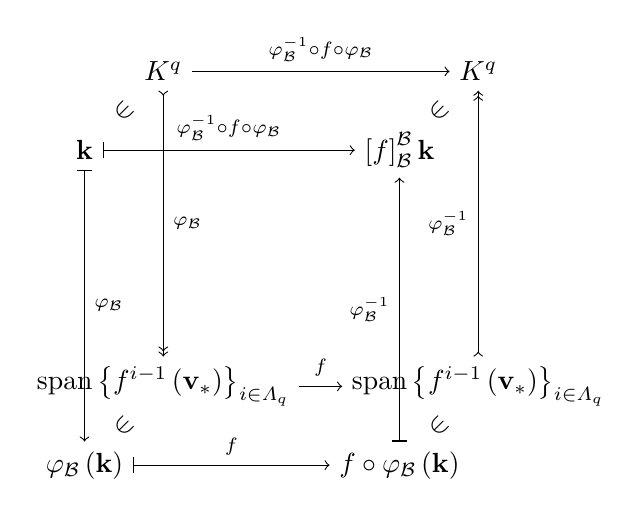
\begin{tikzpicture}[auto]

    \node (a) at (1, 1) {${\rm span} \left\{ f^{i-1} \left( {\bf v}_* \right) \right\}_{i\in \varLambda _q } $};
    \node (b) at (5, 1) {${\rm span} \left\{ f^{i-1} \left( {\bf v}_* \right) \right\}_{i\in \varLambda _q } $};
    \node (c) at (1, 5) {$K^q $};
    \node (d) at (5, 5) {$K^q $};
    \node (e) at (0, 4) {${\bf k} $};
    \node (f) at (4, 4) {$\left[ f\right]_{\mathcal B}^{\mathcal B} {\bf k} $};
    \node (g) at (0.5, 4.5) {\rotatebox{45}{$\scriptsize \in $} };
    \node (h) at (4.5, 4.5) {\rotatebox{45}{$\scriptsize \in $} };
    \node (i) at (0, 0) {$\varphi_{\mathcal B} \left( {\bf k} \right) $};
    \node (j) at (4, 0) {$f\circ \varphi_{\mathcal B} \left( {\bf k} \right) $};
    \node (k) at (0.5, 0.5) {\rotatebox{45}{$\in $} };
    \node (l) at (4.5, 0.5) {\rotatebox{45}{$\in $} };
    
    \draw [->] (c) to node {$\scriptstyle \varphi^{-1}_{\mathcal B} \circ f\circ \varphi_{\mathcal B} $} (d);
    \draw [|->] (e) to node {$\scriptstyle \varphi^{-1}_{\mathcal B} \circ f\circ \varphi_{\mathcal B} $} (f);
    \draw [>->>] (c) to node {$\scriptstyle \varphi_{\mathcal B} $} (a);
    \draw [|->] (e) to node {$\scriptstyle \varphi_{\mathcal B} $} (i);
    \draw [->] (a) to node {$\scriptstyle f$} (b);
    \draw [|->] (i) to node {$\scriptstyle f$} (j);
    \draw [>->>] (b) to node {$\scriptstyle \varphi_{\mathcal B}^{-1} $} (d);
    \draw [|->] (j) to node {$\scriptstyle \varphi_{\mathcal B}^{-1} $} (f);
    
  \end{tikzpicture} 
\end{center}
次のようになる。
\begin{align*}
\varphi_{\mathcal{B}}^{- 1} \circ f \circ \varphi_{\mathcal{B}}\left( \mathbf{k} \right) &= \varphi_{\mathcal{B}}^{- 1} \circ f\left( \sum_{i \in \varLambda_{q}} {k_{i}f^{q - i}\left( \mathbf{v}_{*} \right)} \right)\\
&= \varphi_{\mathcal{B}}^{- 1}\left( \sum_{i \in \varLambda_{q}} {k_{i}f^{q - i + 1}\left( \mathbf{v}_{*} \right)} \right)\\
&= \varphi_{\mathcal{B}}^{- 1}\left( k_{1}f^{q}\left( \mathbf{v}_{*} \right) + \sum_{i \in \varLambda_{q} \setminus \left\{ 1 \right\}} {k_{i}f^{q - i + 1}\left( \mathbf{v}_{*} \right)} \right)\\
&= \varphi_{\mathcal{B}}^{- 1}\left( \sum_{i \in \varLambda_{q} \setminus \left\{ 1 \right\}} {k_{i}f^{q - i + 1}\left( \mathbf{v}_{*} \right)} \right)\\
&= \sum_{i \in \varLambda_{q} \setminus \left\{ 1 \right\}} {k_{i}\varphi_{\mathcal{B}}^{- 1}\left( f^{q - i + 1}\left( \mathbf{v}_{*} \right) \right)}\\
&= k_{1}\mathbf{0} + \sum_{i \in \varLambda_{q} \setminus \left\{ 1 \right\}} {k_{i}\varphi_{\mathcal{B}}^{- 1}\left( f^{q - i + 1}\left( \mathbf{v}_{*} \right) \right)}\\
&= k_{1}\begin{pmatrix}
0 \\
0 \\
 \vdots \\
0 \\
0 \\
\end{pmatrix} + k_{2}\begin{pmatrix}
1 \\
0 \\
 \vdots \\
0 \\
0 \\
\end{pmatrix} + k_{3}\begin{pmatrix}
0 \\
1 \\
 \vdots \\
0 \\
0 \\
\end{pmatrix} + \cdots + k_{q}\begin{pmatrix}
0 \\
0 \\
 \vdots \\
1 \\
0 \\
\end{pmatrix}\\
&= \begin{pmatrix}
0 & 1 & \  & \  & O \\
\  & 0 & 1 & \  & \  \\
\  & \  & 0 & \ddots & \  \\
\  & \  & \  & \ddots & 1 \\
O & \  & \  & \  & 0 \\
\end{pmatrix}\begin{pmatrix}
k_{1} \\
k_{2} \\
k_{3} \\
 \vdots \\
k_{q} \\
\end{pmatrix}\\
&= J(0,q)\mathbf{k}
\end{align*}
したがって、その行列$[ f]_{\mathcal{B}}^{\mathcal{B}}$は$[ f]_{\mathcal{B}}^{\mathcal{B}} = J(0,q)$を満たす。
\end{proof}
\begin{thm}\label{2.2.5.9}
体$K$上の$n$次元vector空間$V$における指数$q$の冪零変換$f:V \rightarrow V$が与えられたとき、その冪零変換$f$の不変系$\left( q_{i} \right)_{i \in \varLambda_{r}}$を用いれば、ある基底$\mathcal{B}$が存在してこれに関するその冪零変換$f$の表現行列$[ f]_{\mathcal{B}}^{\mathcal{B}}$が次式のように表されることができる。
\begin{align*}
[ f]_{\mathcal{B}}^{\mathcal{B}} = \begin{pmatrix}
J\left( 0,q_{1} \right) & \  & \  & O \\
\  & J\left( 0,q_{2} \right) & \  & \  \\
\  & \  & \ddots & \  \\
O & \  & \  & J\left( 0,q_{r} \right) \\
\end{pmatrix}
\end{align*}
さらに、このときの基底$\mathcal{B}$は、$\forall i \in \varLambda_{r}$に対し、$f^{q_{i}}\mathbf{v}_{i} = \mathbf{0}$かつ$f^{q_{i} - 1}\left( \mathbf{v}_{i} \right) \neq \mathbf{0}$なるvectors$\mathbf{v}_{i}$を用いて次式のように表される。
\begin{align*}
\mathcal{B} =\left\langle \begin{matrix}
\mathbf{v}_{1} & \mathbf{v}_{2} & \cdots & \mathbf{v}_{r} \\
f\left( \mathbf{v}_{1} \right) & f\left( \mathbf{v}_{2} \right) & \cdots & f\left( \mathbf{v}_{r} \right) \\
 \vdots & \vdots & \ddots & \vdots \\
f^{q_{1} - 1}\left( \mathbf{v}_{1} \right) & f^{q_{2} - 1}\left( \mathbf{v}_{2} \right) & \cdots & f^{q_{r} - 1}\left( \mathbf{v}_{r} \right) \\
\end{matrix} \right\rangle
\end{align*}
逆に、このような基底$\mathcal{B}$が存在するようなそのvector空間$V$における線形写像$f:V \rightarrow V$は不変系$\left( q_{i} \right)_{i \in \varLambda_{r}}$の冪零変換である。
\end{thm}
\begin{proof}
体$K$上の$n$次元vector空間$V$における指数$q$の冪零変換$f:V \rightarrow V$が与えられたとき、その冪零変換$f$の不変系$\left( q_{i} \right)_{i \in \varLambda_{r}}$を用いれば、定理\ref{2.2.1.6}、定理\ref{2.2.5.3}より次式が成り立つ。
\begin{align*}
V = \bigoplus_{j \in \varLambda_{r}} {{\mathrm{span}}\left\{ f^{i - 1}\left( \mathbf{v}_{j} \right) \right\}_{i \in \varLambda_{q_{j}}}}
\end{align*}
定理\ref{2.2.5.8}よりそれらの部分空間たち${\mathrm{span}}\left\{ f^{i - 1}\left( \mathbf{v}_{j} \right) \right\}_{i \in \varLambda_{q_{j}}}$は$f$-不変でこれの基底$\mathcal{B}_{j}$が$\left\langle f^{q_{j} - i}\left( \mathbf{v}_{j} \right) \right\rangle_{i \in \varLambda_{q_{j}}}$とおかれると、これに関する表現行列$[ f]_{\mathcal{B}_{j}}^{\mathcal{B}_{j}}$は$[ f]_{\mathcal{B}_{j}}^{\mathcal{B}_{j}} = J\left( 0,q_{j} \right)$を満たす。このとき、$\forall\mathbf{k} \in V$に対し、基底$\left\langle \mathcal{B}_{j} \right\rangle_{j \in \varLambda_{r}}$が$\mathcal{B}$とおかれその基底$\mathcal{B}$に関する基底変換における線形同型写像$\varphi_{\mathcal{B}}:K^{n} \rightarrow V$を用いて$\varphi_{\mathcal{B}}^{- 1}\left( \mathbf{k} \right) = \bigoplus_{j \in \varLambda_{r}} \mathbf{w}_{j}$とおくと、これに関する表現行列$[ f]_{\mathcal{B}}^{\mathcal{B}}$について、次のようになる。
\begin{center}
  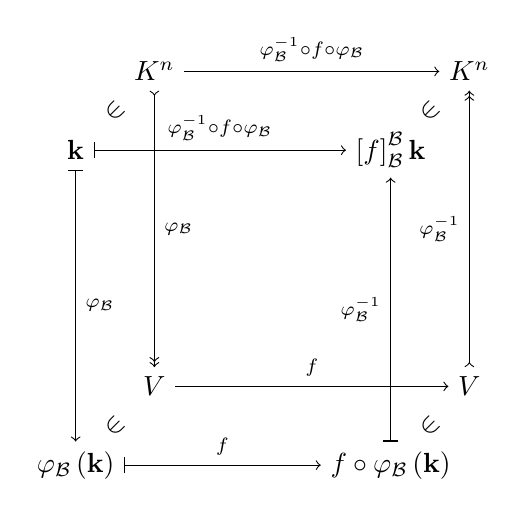
\begin{tikzpicture}[auto]

    \node (a) at (1, 1) {$V$};
    \node (b) at (5, 1) {$V$};
    \node (c) at (1, 5) {$K^n $};
    \node (d) at (5, 5) {$K^n $};
    \node (e) at (0, 4) {${\bf k} $};
    \node (f) at (4, 4) {$\left[ f\right] _{\mathcal B}^{\mathcal B} {\bf k} $};
    \node (g) at (0.5, 4.5) {\rotatebox{45}{$\scriptsize \in $} };
    \node (h) at (4.5, 4.5) {\rotatebox{45}{$\scriptsize \in $} };
    \node (i) at (0, 0) {$\varphi_{\mathcal B} \left( {\bf k} \right) $};
    \node (j) at (4, 0) {$f\circ \varphi_{\mathcal B} \left( {\bf k} \right) $};
    \node (k) at (0.5, 0.5) {\rotatebox{45}{$\in $} };
    \node (l) at (4.5, 0.5) {\rotatebox{45}{$\in $} };
    
    \draw [->] (c) to node {$\scriptstyle \varphi_{\mathcal B}^{-1} \circ f\circ \varphi_{\mathcal B} $} (d);
    \draw [|->] (e) to node {$\scriptstyle \varphi_{\mathcal B}^{-1} \circ f\circ \varphi_{\mathcal B} $} (f);
    \draw [>->>] (c) to node {$\scriptstyle \varphi_{\mathcal B} $} (a);
    \draw [|->] (e) to node {$\scriptstyle \varphi_{\mathcal B} $} (i);
    \draw [->] (a) to node {$\scriptstyle f $} (b);
    \draw [|->] (i) to node {$\scriptstyle f $} (j);
    \draw [>->>] (b) to node {$\scriptstyle \varphi_{\mathcal B}^{-1} $} (d);
    \draw [|->] (j) to node {$\scriptstyle \varphi_{\mathcal B}^{-1} $} (f);
    
  \end{tikzpicture} 
\end{center}
したがって、次のようになる。
\begin{align*}
\varphi_{\mathcal{B}}^{- 1} \circ f \circ \varphi_{\mathcal{B}}\left( \mathbf{k} \right) &= \varphi_{\mathcal{B}}^{- 1} \circ f\left( \bigoplus_{j \in \varLambda_{r}} \mathbf{w}_{j} \right)\\
&= \sum_{j \in \varLambda_{r}} {\varphi_{\mathcal{B}}^{- 1} \circ f\left( \mathbf{w}_{j} \right)}\\
&= \begin{pmatrix}
\varphi_{\mathcal{B}_{1}}^{- 1} \circ f\left( \mathbf{w}_{1} \right) \\
\mathbf{0} \\
 \vdots \\
\mathbf{0} \\
\end{pmatrix} + \begin{pmatrix}
\mathbf{0} \\
\varphi_{\mathcal{B}_{2}}^{- 1} \circ f\left( \mathbf{w}_{2} \right) \\
 \vdots \\
\mathbf{0} \\
\end{pmatrix} + \cdots + \begin{pmatrix}
\mathbf{0} \\
\mathbf{0} \\
 \vdots \\
\varphi_{\mathcal{B}_{r}}^{- 1} \circ f\left( \mathbf{w}_{r} \right) \\
\end{pmatrix}\\
&= \begin{pmatrix}
\varphi_{\mathcal{B}_{1}}^{- 1} \circ f \circ \varphi_{\mathcal{B}_{1}} \circ \varphi_{\mathcal{B}_{1}}^{- 1}\left( \mathbf{w}_{1} \right) \\
\mathbf{0} \\
 \vdots \\
\mathbf{0} \\
\end{pmatrix} + \begin{pmatrix}
\mathbf{0} \\
\varphi_{\mathcal{B}_{2}}^{- 1} \circ f \circ \varphi_{\mathcal{B}_{2}} \circ \varphi_{\mathcal{B}_{2}}^{- 1}\left( \mathbf{w}_{2} \right) \\
 \vdots \\
\mathbf{0} \\
\end{pmatrix} + \cdots + \begin{pmatrix}
\mathbf{0} \\
\mathbf{0} \\
 \vdots \\
\varphi_{\mathcal{B}_{r}}^{- 1} \circ f \circ \varphi_{\mathcal{B}_{r}} \circ \varphi_{\mathcal{B}_{r}}^{- 1}\left( \mathbf{w}_{r} \right) \\
\end{pmatrix}\\
&= \begin{pmatrix}
[ f]_{\mathcal{B}_{1}}^{\mathcal{B}_{1}}\varphi_{\mathcal{B}_{1}}^{- 1}\left( \mathbf{w}_{1} \right) \\
\mathbf{0} \\
 \vdots \\
\mathbf{0} \\
\end{pmatrix} + \begin{pmatrix}
\mathbf{0} \\
[ f]_{\mathcal{B}_{2}}^{\mathcal{B}_{2}}\varphi_{\mathcal{B}_{2}}^{- 1}\left( \mathbf{w}_{2} \right) \\
 \vdots \\
\mathbf{0} \\
\end{pmatrix} + \cdots + \begin{pmatrix}
\mathbf{0} \\
\mathbf{0} \\
 \vdots \\
[ f]_{\mathcal{B}_{r}}^{\mathcal{B}_{r}}\varphi_{\mathcal{B}_{r}}^{- 1}\left( \mathbf{w}_{r} \right) \\
\end{pmatrix}\\
&= \begin{pmatrix}
[ f]_{\mathcal{B}_{1}}^{\mathcal{B}_{1}} \\
O \\
 \vdots \\
O \\
\end{pmatrix}\varphi_{\mathcal{B}_{1}}^{- 1}\left( \mathbf{w}_{1} \right) + \begin{pmatrix}
O \\
[ f]_{\mathcal{B}_{2}}^{\mathcal{B}_{2}} \\
 \vdots \\
O \\
\end{pmatrix}\varphi_{\mathcal{B}_{2}}^{- 1}\left( \mathbf{w}_{2} \right) + \cdots + \begin{pmatrix}
O \\
O \\
 \vdots \\
[ f]_{\mathcal{B}_{r}}^{\mathcal{B}_{r}} \\
\end{pmatrix}\varphi_{\mathcal{B}_{r}}^{- 1}\left( \mathbf{w}_{r} \right)\\
&= \begin{pmatrix}
J\left( 0,q_{1} \right) \\
O \\
 \vdots \\
O \\
\end{pmatrix}\varphi_{\mathcal{B}_{1}}^{- 1}\left( \mathbf{w}_{1} \right) + \begin{pmatrix}
O \\
J\left( 0,q_{2} \right) \\
 \vdots \\
O \\
\end{pmatrix}\varphi_{\mathcal{B}_{2}}^{- 1}\left( \mathbf{w}_{2} \right) + \cdots + \begin{pmatrix}
O \\
O \\
 \vdots \\
J\left( 0,q_{r} \right) \\
\end{pmatrix}\varphi_{\mathcal{B}_{r}}^{- 1}\left( \mathbf{w}_{r} \right)\\
&= \begin{pmatrix}
J\left( 0,q_{1} \right) & \  & \  & O \\
\  & J\left( 0,q_{2} \right) & \  & \  \\
\  & \  & \ddots & \  \\
O & \  & \  & J\left( 0,q_{r} \right) \\
\end{pmatrix}\begin{pmatrix}
\varphi_{\mathcal{B}_{1}}^{- 1}\left( \mathbf{w}_{1} \right) \\
\varphi_{\mathcal{B}_{2}}^{- 1}\left( \mathbf{w}_{2} \right) \\
 \vdots \\
\varphi_{\mathcal{B}_{r}}^{- 1}\left( \mathbf{w}_{r} \right) \\
\end{pmatrix}
\end{align*}
ここで、次のようになるので、
\begin{align*}
\begin{pmatrix}
\varphi_{\mathcal{B}_{1}}^{- 1}\left( \mathbf{w}_{1} \right) \\
\varphi_{\mathcal{B}_{2}}^{- 1}\left( \mathbf{w}_{2} \right) \\
 \vdots \\
\varphi_{\mathcal{B}_{r}}^{- 1}\left( \mathbf{w}_{r} \right) \\
\end{pmatrix} &= \begin{pmatrix}
\varphi_{\mathcal{B}_{1}}^{- 1}\left( \mathbf{w}_{1} \right) \\
\mathbf{0} \\
 \vdots \\
\mathbf{0} \\
\end{pmatrix} + \begin{pmatrix}
\mathbf{0} \\
\varphi_{\mathcal{B}_{2}}^{- 1}\left( \mathbf{w}_{2} \right) \\
 \vdots \\
\mathbf{0} \\
\end{pmatrix} + \cdots + \begin{pmatrix}
\mathbf{0} \\
\mathbf{0} \\
 \vdots \\
\varphi_{\mathcal{B}_{r}}^{- 1}\left( \mathbf{w}_{r} \right) \\
\end{pmatrix}\\
&= \varphi_{\mathcal{B}}^{- 1}\left( \mathbf{w}_{1} \right) + \varphi_{\mathcal{B}}^{- 1}\left( \mathbf{w}_{2} \right) + \cdots + \varphi_{\mathcal{B}}^{- 1}\left( \mathbf{w}_{r} \right)\\
&= \varphi_{\mathcal{B}}^{- 1}\left( \bigoplus_{j \in \varLambda_{r}} \mathbf{w}_{j} \right)\\
&= \varphi_{\mathcal{B}}^{- 1}\left( \mathbf{v} \right) = \mathbf{k}
\end{align*}
次のようになる。
\begin{align*}
\varphi_{\mathcal{B}}^{- 1} \circ f \circ \varphi_{\mathcal{B}}\left( \mathbf{k} \right) = \begin{pmatrix}
J\left( 0,q_{1} \right) & \  & \  & O \\
\  & J\left( 0,q_{2} \right) & \  & \  \\
\  & \  & \ddots & \  \\
O & \  & \  & J\left( 0,q_{r} \right) \\
\end{pmatrix}\mathbf{k}
\end{align*}
ゆえに、ある基底$\mathcal{B}$が存在してこれに関するその冪零変換$f$の表現行列$[ f]_{\mathcal{B}}^{\mathcal{B}}$が次式のように表されることができる。
\begin{align*}
[ f]_{\mathcal{B}}^{\mathcal{B}} = \begin{pmatrix}
J\left( 0,q_{1} \right) & \  & \  & O \\
\  & J\left( 0,q_{2} \right) & \  & \  \\
\  & \  & \ddots & \  \\
O & \  & \  & J\left( 0,q_{r} \right) \\
\end{pmatrix}
\end{align*}\par
さらに、このときの基底$\mathcal{B}$は上記の議論により、$\forall i \in \varLambda_{r}$に対し、$f^{q_{i}}\mathbf{v}_{i} = \mathbf{0}$かつ$f^{q_{i} - 1}\left( \mathbf{v}_{i} \right) \neq \mathbf{0}$なるvectors$\mathbf{v}_{i}$を用いて次式のように表される。
\begin{align*}
\mathcal{B} &= \left\langle \mathcal{B}_{j} \right\rangle_{j \in \varLambda_{r}}\\
&= \left\langle f^{q_{j} - i}\left( \mathbf{v}_{j} \right) \right\rangle_{(i,j) \in \varLambda_{q_{j}} \times \varLambda_{r}}\\
&= \left\langle \begin{matrix}
\mathbf{v}_{1} & \mathbf{v}_{2} & \cdots & \mathbf{v}_{r} \\
f\left( \mathbf{v}_{1} \right) & f\left( \mathbf{v}_{2} \right) & \cdots & f\left( \mathbf{v}_{r} \right) \\
 \vdots & \vdots & \ddots & \vdots \\
f^{q_{1} - 1}\left( \mathbf{v}_{1} \right) & f^{q_{2} - 1}\left( \mathbf{v}_{2} \right) & \cdots & f^{q_{r} - 1}\left( \mathbf{v}_{r} \right) \\
\end{matrix} \right\rangle
\end{align*}\par
逆に、ある基底$\mathcal{B}$が存在して、$\forall j \in \varLambda_{r - 1}$に対し、$q_{j + 1} \leq q_{j}$が成り立つかつ、これに関する線形写像$f:V \rightarrow V$の表現行列$[ f]_{\mathcal{B}}^{\mathcal{B}}$が次式のように表されることができるなら、
\begin{align*}
[ f]_{\mathcal{B}}^{\mathcal{B}} = \begin{pmatrix}
J\left( 0,q_{1} \right) & \  & \  & O \\
\  & J\left( 0,q_{2} \right) & \  & \  \\
\  & \  & \ddots & \  \\
O & \  & \  & J\left( 0,q_{r} \right) \\
\end{pmatrix}
\end{align*}
定理\ref{2.2.1.6}より$\mathcal{B} =\left\langle \mathcal{B}_{j} \right\rangle_{j \in \varLambda_{r}}$なる基底$\mathcal{B}_{j}$をもつ$q_{j}$次元のそのvector空間$V$の部分空間たち$W_{j}$を用いて次式が成り立つのであった。
\begin{align*}
V = \bigoplus_{j \in \varLambda_{r}} W_{j}
\end{align*}
このとき、$\forall j \in \varLambda_{r}$に対し、その部分空間$W_{j}$の基底$\mathcal{B}_{j}$が$\left\langle \mathbf{w}_{ij} \right\rangle_{i \in \varLambda_{q_{j}}}$とおかれると、次のようになることにより、
\begin{center}
  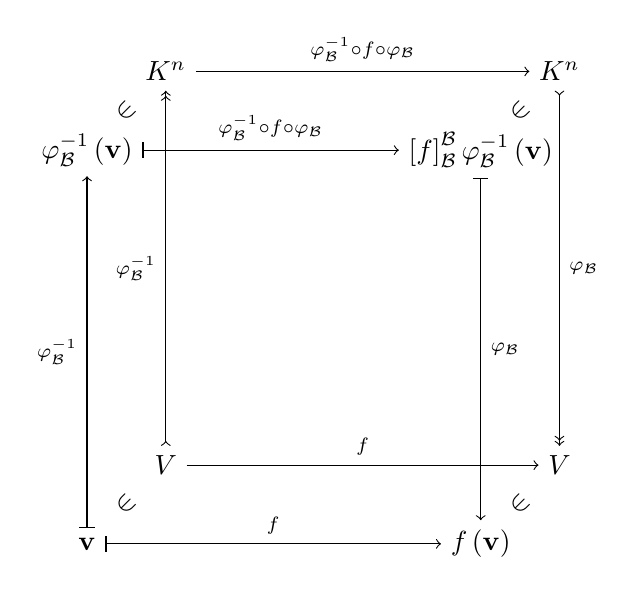
\begin{tikzpicture}[auto]

    \node (a) at (1, 1) {$V$};
    \node (b) at (6, 1) {$V$};
    \node (c) at (1, 6) {$K^n $};
    \node (d) at (6, 6) {$K^n $};
    \node (e) at (0, 5) {$\varphi_{\mathcal B}^{-1} \left( {\bf v} \right) $};
    \node (f) at (5, 5) {$\left[ f\right] _{\mathcal B}^{\mathcal B} \varphi_{\mathcal B}^{-1} \left( {\bf v} \right) $};
    \node (g) at (0.5, 5.5) {\rotatebox{45}{$\scriptsize \in $} };
    \node (h) at (5.5, 5.5) {\rotatebox{45}{$\scriptsize \in $} };
    \node (i) at (0, 0) {${\bf v} $};
    \node (j) at (5, 0) {$f\left( {\bf v} \right) $};
    \node (k) at (0.5, 0.5) {\rotatebox{45}{$\in $} };
    \node (l) at (5.5, 0.5) {\rotatebox{45}{$\in $} };
    
    \draw [->] (c) to node {$\scriptstyle \varphi_{\mathcal B}^{-1} \circ f\circ \varphi_{\mathcal B} $} (d);
    \draw [|->] (e) to node {$\scriptstyle \varphi_{\mathcal B}^{-1} \circ f\circ \varphi_{\mathcal B} $} (f);
    \draw [>->>] (a) to node {$\scriptstyle \varphi_{\mathcal B}^{-1} $} (c);
    \draw [|->] (i) to node {$\scriptstyle \varphi_{\mathcal B}^{-1} $} (e);
    \draw [->] (a) to node {$\scriptstyle f $} (b);
    \draw [|->] (i) to node {$\scriptstyle f $} (j);
    \draw [>->>] (d) to node {$\scriptstyle \varphi_{\mathcal B} $} (b);
    \draw [|->] (f) to node {$\scriptstyle \varphi_{\mathcal B} $} (j);
    
  \end{tikzpicture} 
\end{center}
次のようになり、
\begin{align*}
f\left( \mathbf{w}_{ij} \right) &= \varphi_{\mathcal{B}} \circ \varphi_{\mathcal{B}}^{- 1} \circ f \circ \varphi_{\mathcal{B}} \circ \varphi_{\mathcal{B}}^{- 1}\left( \mathbf{w}_{ij} \right)\\
&= \varphi_{\mathcal{B}}\left( [ f]_{\mathcal{B}}^{\mathcal{B}}\varphi_{\mathcal{B}}^{- 1}\left( \mathbf{w}_{ij} \right) \right)\\
&= \varphi_{\mathcal{B}}\left( \begin{pmatrix}
J\left( 0,q_{1} \right) & \  & \  & \  & O \\
\  & \ddots & \  & \  & \  \\
\  & \  & J\left( 0,q_{j} \right) & \  & \  \\
\  & \  & \  & \ddots & \  \\
O & \  & \  & \  & J\left( 0,q_{r} \right) \\
\end{pmatrix}\begin{pmatrix}
\mathbf{0} \\
 \vdots \\
\varphi_{\mathcal{B}_{j}}^{- 1}\left( \mathbf{w}_{ij} \right) \\
 \vdots \\
\mathbf{0} \\
\end{pmatrix} \right)\\
&= \varphi_{\mathcal{B}}\begin{pmatrix}
\mathbf{0} \\
 \vdots \\
J\left( 0,q_{j} \right)\varphi_{\mathcal{B}_{j}}^{- 1}\left( \mathbf{w}_{ij} \right) \\
 \vdots \\
\mathbf{0} \\
\end{pmatrix}
\end{align*}
ここで、$i = 1$のとき、次のようになるかつ、
\begin{align*}
J\left( 0,q_{j} \right)\varphi_{\mathcal{B}_{j}}^{- 1}\left( \mathbf{w}_{1j} \right) = \begin{pmatrix}
0 & 1 & \  & \  & O \\
\  & 0 & 1 & \  & \  \\
\  & \  & 0 & \ddots & \  \\
\  & \  & \  & \ddots & 1 \\
O & \  & \  & \  & 0 \\
\end{pmatrix}\begin{pmatrix}
1 \\
0 \\
0 \\
 \vdots \\
0 \\
\end{pmatrix} = \begin{pmatrix}
0 \\
0 \\
0 \\
 \vdots \\
0 \\
\end{pmatrix} = \varphi_{\mathcal{B}_{j}}^{- 1}\left( \mathbf{0} \right)
\end{align*}
$i > 1$のとき、次のようになることから、
\begin{align*}
J\left( 0,q_{j} \right)\varphi_{\mathcal{B}_{j}}^{- 1}\left( \mathbf{w}_{ij} \right) = \begin{pmatrix}
0 & \ddots & \  & \  & \  & O \\
\  & \ddots & 1 & \  & \  & \  \\
\  & \  & 0 & 1 & \  & \  \\
\  & \  & \  & 0 & \ddots & \  \\
\  & \  & \  & \  & \ddots & 1 \\
O & \  & \  & \  & \  & 0 \\
\end{pmatrix}\begin{pmatrix}
0 \\
 \vdots \\
0 \\
1 \\
 \vdots \\
0 \\
\end{pmatrix} = \begin{pmatrix}
0 \\
 \vdots \\
1 \\
0 \\
 \vdots \\
0 \\
\end{pmatrix} = \varphi_{\mathcal{B}_{j}}^{- 1}\left( \mathbf{w}_{i - 1,j} \right)
\end{align*}
次式が成り立つ。
\begin{align*}
f\left( \mathbf{w}_{ij} \right) &= \left\{ \begin{matrix}
\varphi_{\mathcal{B}}\begin{pmatrix}
\mathbf{0} \\
 \vdots \\
\varphi_{\mathcal{B}_{j}}^{- 1}\left( \mathbf{0} \right) \\
 \vdots \\
\mathbf{0} \\
\end{pmatrix} & \mathrm{if} & i = 1 \\
\varphi_{\mathcal{B}}\begin{pmatrix}
\mathbf{0} \\
 \vdots \\
\varphi_{\mathcal{B}_{j}}^{- 1}\left( \mathbf{w}_{i - 1,j} \right) \\
 \vdots \\
\mathbf{0} \\
\end{pmatrix} & \mathrm{if} & i > 1 \\
\end{matrix} \right.\ \\
&= \left\{ \begin{matrix}
\varphi_{\mathcal{B}} \circ \varphi_{\mathcal{B}}^{- 1}\left( \mathbf{0} \right) & \mathrm{if} & i = 1 \\
\varphi_{\mathcal{B}} \circ \varphi_{\mathcal{B}}^{- 1}\begin{pmatrix}
\mathbf{w}_{i - 1,j} \\
\end{pmatrix} & \mathrm{if} & i > 1 \\
\end{matrix} \right.\ \\
&= \left\{ \begin{matrix}
\mathbf{0} & \mathrm{if} & i = 1 \\
\mathbf{w}_{i - 1,j} & \mathrm{if} & i > 1 \\
\end{matrix} \right.\ 
\end{align*}
このとき、数学的帰納法により、$f^{q_{j}}\left( \mathbf{w}_{q_{j}j} \right) = \mathbf{0}$、$i > 1$のとき、$f^{q_{j} - i + 1}\left( \mathbf{w}_{q_{j}j} \right) = \mathbf{w}_{i - 1,j}$が成り立つので、$q_{j} \leq q_{1}$より$q = q_{1}$とおかれると、その線形写像$f$は指数$q$の冪零変換であり、さらに、その部分空間$W_{j}$の基底が$\left\langle f^{q_{j} - i + 1}\left( \mathbf{w}_{q_{j}j} \right) \right\rangle_{i \in \varLambda_{q_{j} + 1} \setminus \left\{ 1 \right\}}$、即ち、$\left\langle f^{q_{j} - i}\left( \mathbf{w}_{q_{j}j} \right) \right\rangle_{i \in \varLambda_{q_{j}}}$と与えられる。以上、次のことを満たすそのvector空間$V$の元の列$\left( \mathbf{v}_{j} \right)_{j \in \varLambda_{r}}$と自然数の列$\left( q_{j} \right)_{j \in \varLambda_{r}}$が存在する。
\begin{itemize}
\item
  $q_{1} = q$が成り立つかつ、$\forall j \in \varLambda_{r - 1}$に対し、$q_{j + 1} \leq q_{j}$が成り立つ。
\item
  $\sum_{j \in \varLambda_{r}} q_{j} = n$が成り立つ。
\item
  次式のような$n$つのvectorsの組$\mathcal{B}$はそのvector空間$V$の基底をなす。
\begin{align*}
\alpha = \left\langle \begin{matrix}
\mathbf{v}_{1} & \mathbf{v}_{2} & \cdots & \mathbf{v}_{r} \\
f\left( \mathbf{v}_{1} \right) & f\left( \mathbf{v}_{2} \right) & \cdots & f\left( \mathbf{v}_{r} \right) \\
 \vdots & \vdots & \ddots & \vdots \\
f^{q_{1} - 1}\left( \mathbf{v}_{1} \right) & f^{q_{2} - 1}\left( \mathbf{v}_{2} \right) & \cdots & f^{q_{r} - 1}\left( \mathbf{v}_{r} \right) \\
\end{matrix} \right\rangle
\end{align*}
\item
  $\forall j \in \varLambda_{r}$に対し、$f^{q_{j}}\left( \mathbf{v}_{j} \right) = \mathbf{0}$が成り立つ。
\end{itemize}
よって、このような基底$\mathcal{B}$が存在するようなそのvector空間$V$における線形写像$f:V \rightarrow V$は不変系$\left( q_{i} \right)_{i \in \varLambda_{r}}$の冪零変換である。
\end{proof}
\begin{thebibliography}{50}
  \bibitem{1}
    松坂和夫, 線型代数入門, 岩波書店, 1980. 新装版第2刷 p276-288 ISBN978-4-00-029872-8
\end{thebibliography}
\end{document}
